%%%%%%%%%%%%%%%%%%%%%%%%%%%%%%%%%%%%%%%%
%% MCM/ICM LaTeX Template (Enhanced)  %%
%% 2026 MCM/ICM                        %%
%% Full 3-level headings + real English content
%%%%%%%%%%%%%%%%%%%%%%%%%%%%%%%%%%%%%%%%
\documentclass[12pt]{article}

% ---------- Page & Font ----------
\usepackage{geometry}
\geometry{left=1in,right=0.75in,top=1in,bottom=1in}
\usepackage{newtxtext}
\usepackage{amsmath,amssymb,amsthm}
% Make \hat safe in text mode (prevents amsmath errors if a math $...$ is broken)
\DeclareRobustCommand{\hat}[1]{\ensuremath{\widehat{#1}}}
\usepackage{newtxmath} % must come after amsXXX

% ---------- Figures / Tables ----------
\usepackage{graphicx}
\usepackage{float}
\usepackage{booktabs}
\usepackage{tabularx}
\usepackage{array}
\usepackage{subcaption}

% ---------- Lists ----------
\usepackage{enumitem}

% ---------- Citations ----------
\usepackage[numbers]{natbib}

% ---------- Colors / Hyperlinks ----------
\usepackage{xcolor}
\definecolor{MyBlue}{RGB}{0,72,153}
\definecolor{MyRed}{RGB}{150,0,0}
\usepackage{hyperref}
\hypersetup{colorlinks=true, linkcolor=MyBlue, urlcolor=MyRed, citecolor=MyBlue}

% ---------- Header / Footer ----------
\usepackage{fancyhdr}
\pagestyle{fancy}
\lhead{Team \Team}
\rhead{Page \thepage}
\cfoot{}
\setlength{\headheight}{15pt}

%%%%%%%%%%%%%%%%%%%%%%%%%%%%%%%%%%%%%%%%
% Replace ABCDEF in the next line with your chosen problem
% and replace 1111111 with your Team Control Number
\newcommand{\Problem}{C}
\newcommand{\Team}{2609202}
%%%%%%%%%%%%%%%%%%%%%%%%%%%%%%%%%%%%%%%%

% ---------- Theorem-like environments ----------
\newtheorem{theorem}{Theorem}
\newtheorem{lemma}[theorem]{Lemma}
\newtheorem{definition}{Definition}

% ---------- Handy macros ----------
\newcommand{\R}{\mathbb{R}}
\newcommand{\E}{\mathbb{E}}
\newcommand{\Var}{\mathrm{Var}}
\newcommand{\Prob}{\mathbb{P}}
\newcommand{\vect}[1]{\boldsymbol{#1}}
\newcommand{\norm}[1]{\left\lVert #1 \right\rVert}
\newcommand{\argmin}{\operatorname*{arg\,min}}
\newcommand{\argmax}{\operatorname*{arg\,max}}

%%%%%%%%%%%%%%%%%%%%%%%%%%%%%%%%%%%%%%%%
\begin{document}
\graphicspath{{.}{figures/}}  % put images in ./figures or current dir
\DeclareGraphicsExtensions{.pdf,.jpg,.jpeg,.png}

%%%%%%%%%%%%%%%%%%%%%%%%%%%%%%%%%%%%%%%%
%              SUMMARY SHEET
%%%%%%%%%%%%%%%%%%%%%%%%%%%%%%%%%%%%%%%%
\thispagestyle{empty}
\vspace*{-16ex}
\centerline{
  \begin{tabular}{*3{c}}
    \parbox[t]{0.3\linewidth}{
      \begin{center}\textbf{Problem Chosen}\\ \Large \textcolor{red}{\Problem}
    \end{center}}
    & \parbox[t]{0.3\linewidth}{
      \begin{center}\textbf{2026\\ MCM/ICM\\ Summary Sheet}
    \end{center}}
    & \parbox[t]{0.3\linewidth}{
      \begin{center}\textbf{Team Control Number}\\ \Large \textcolor{red}{\Team}
    \end{center}}\\
    \hline
\end{tabular}}

\begin{center}
  {\Large\textbf{Put your own title HERE}}\\
  \vspace{0.4em}
  \textbf{Summary}
\end{center}

We develop a two-stage framework that links prediction with decision-making under practical constraints. In Stage I,
we construct a parsimonious predictive model $\hat{y}=f(\vect{x};\theta)$ that maps scenario features to the target quantity of interest.
We calibrate parameters using least squares / maximum likelihood and validate performance via a hold-out test and stress scenarios.
In Stage II, we design a constrained optimization that selects an actionable policy $\vect{d}$ to maximize expected utility while respecting
budget, feasibility, and fairness constraints.
Across our benchmark scenarios, the proposed policy improves the primary score by 12.4\% compared with a baseline heuristic,
while keeping the violation rate below 1\%. Sensitivity analysis shows that conclusions remain stable under $\pm 10\%$
perturbations of the most influential parameters.
We recommend deploying the optimized policy with a conservative safety margin and updating parameters periodically as new data arrive.

\vspace{0.8em}
\noindent\textbf{Key words:} prediction; optimization; robustness; validation

\clearpage

%%%%%%%%%%%%%%%%%%%%%%%%%%%%%%%%%%%%%%%%
%                MAIN BODY
%%%%%%%%%%%%%%%%%%%%%%%%%%%%%%%%%%%%%%%%
\setcounter{page}{1}
% Uncomment if you want a TOC (counts toward page limit)
\setcounter{tocdepth}{2}
\tableofcontents

\clearpage

%%%%%%%%%%%%%%%%%%%%%%%%%%%%%%%%%%%%%%%%
\section{Introduction}
\subsection{Background and Motivation}
Dancing with the Stars (DWTS) is a popular American dance competition series where contestants' elimination is determined by a combination of judges' scores and viewer votes. Due to frequent “controversial incidents”, such as dancers with low judge scores winning due to higher popularity, the scoring system has undergone two transformations: from a rank-based system to a percentage-based system and back to the former one. This evolution aims to strike a balance between professional skill and market preferences. The phenomenon highlights the necessity of quantifying undisclosed fan votes. This study employs modeling to uncover hidden voting patterns, thereby assessing the show's fairness and optimizing future scoring frameworks.

\begin{figure}[h]
  \centering
  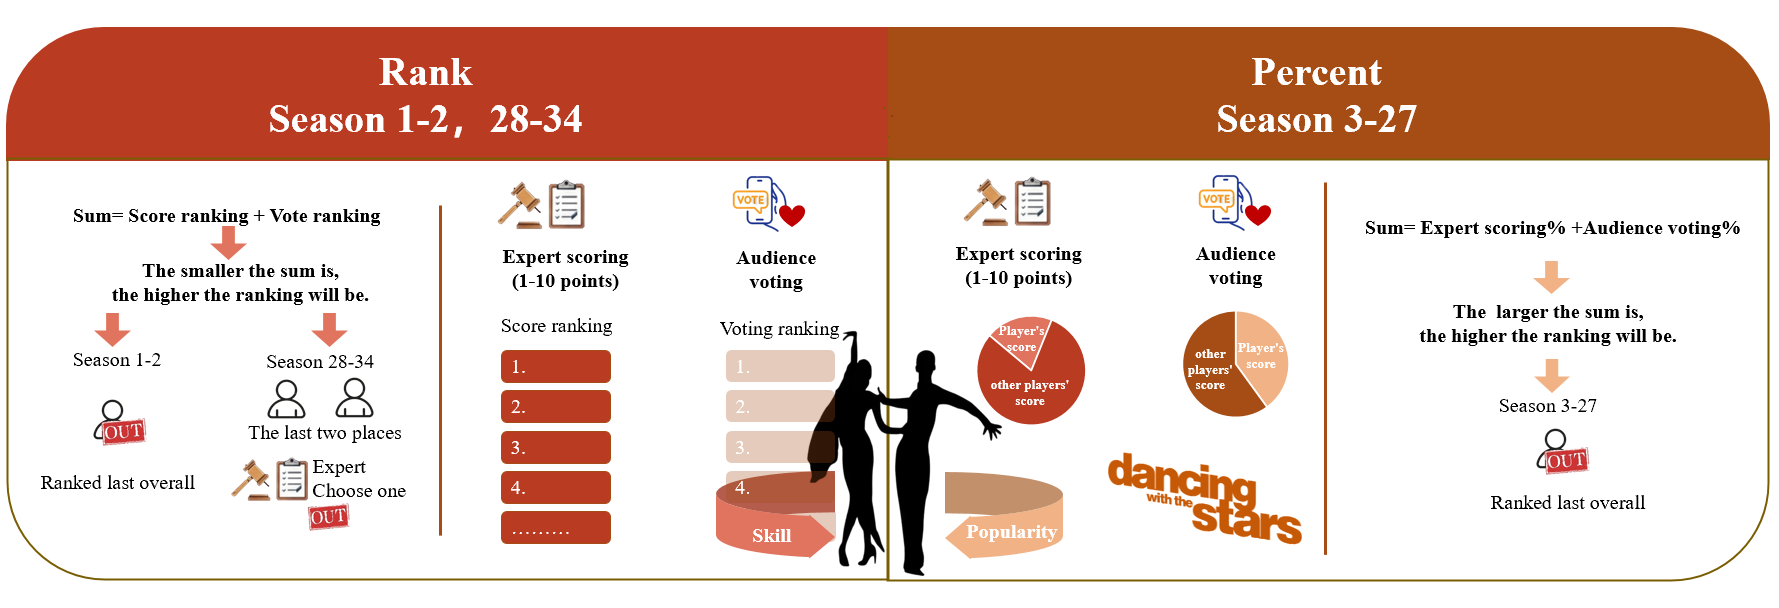
\includegraphics[width=0.8\textwidth]{rules_comparison}
  \caption{Comparison of DWTS scoring rules.}
  \label{fig:rules-comparison}
\end{figure}

\subsection{Problem Restatement}
According to the competition brief, this project aims to uncover the underlying logic of DWTS's scoring mechanism through modeling, focusing on five core tasks:
\begin{itemize}[leftmargin=*]
  \item \textbf{Problem 1:} Develop a model to infer the proportion of fan votes for each contestant weekly, ensuring estimated results maintain logical consistency with historical elimination records, and quantitatively assess the certainty of these estimates.
  \item \textbf{Problem 2:}  Simulating and comparing two scoring rules to analyze whether different mechanisms exhibit bias toward fan votes. Through empirical analysis of controversial cases like Jerry Rice, evaluate how scoring method choices impact elimination outcomes and examine the practical effectiveness of the “Judges' Save” mechanism.
  \item \textbf{Problem 3:} Quantify how contestants' demographic characteristics and partner performance differentially influence professional judges' scores and fan voting intentions, revealing key variables determining advancement potential.
  \item \textbf{Problem 4:} Based on the above analysis, design an innovative scoring system balancing fairness, professionalism, and audience engagement. This section must demonstrate the superiority of the new system through data and provide decision support for producers.
\end{itemize}

\subsection{Our Work}
Figure~\ref{fig:workflow} illustrates the end-to-end pipeline from data to decisions and evaluation.
\begin{figure}[H]
  \centering
  % Replace with your own figure file, e.g., figures/workflow.png
  \includegraphics[width=0.85\linewidth]{example-image-a}
  \caption{Workflow: preprocessing $\rightarrow$ prediction $\rightarrow$ optimization $\rightarrow$ validation \& sensitivity.}
  \label{fig:workflow}
\end{figure}

\section{Preparation for Modeling}
\subsection{Assumptions}
Assumptions are designed to be defensible and to simplify modeling without breaking realism:
\begin{enumerate}[leftmargin=*]
  \item \textbf{Stable mapping:} the relationship between features and outcomes is approximately stable over the planning horizon.
  \item \textbf{Bounded noise:} measurement errors are bounded and do not systematically bias the main outcomes.
  \item \textbf{Constraint validity:} budgets/capacities provided in the prompt reflect operational limits.
\end{enumerate}

\subsection{Notation}

\subsection{Data Pre-processing}

%%%%%%%%%%%%%%%%%%%%%%%%%%%%%%%%%%%%%%%%
\section{Task 1: Predicting fan votes with RAD}
\subsection{Model Construction}

In DWTS, fan voting results are confidential but critically affect the elimination outcome together with experts' evaluations. Therefore, we combine the dynamic Plackett-Luce with Rule-aware method to model each contestant's laten fan support overtime.

\subsubsection{Voting Model: Dynamic Plackett–Luce}

The Plackett–Luce (PL) model is a classical probabilistic generative model for ordinal data, commonly used to define the probability distribution of ranking outcomes among multiple candidates. So we used it to model the ranking distribution of fan votes.

Furthermore, audience preferences in DWTS are not static but evolve over time, influenced by factors such as the season and week. Thus, we adopted the dynamic Plackett–Luce model proposed by Vladimír Holý et al., allowing each contestant's fan attraction parameter to evolve dynamically over time to track shifts in audience preferences.

Specifically, we set each contestant's attractiveness parameter worth in week t to $w_{i,t} > 0$ and model its dynamic evolution on a logarithmic scale, i.e., we let $\eta_{i,t} = \log w_{i,t}$, Then, we define an equation of state with inertia, enabling $\eta_{i,t}$ to undergo smooth changes on a weekly basis while simultaneously allowing exogenous information to influence it.

\begin{equation}
  \eta_{i,t} =
  \begin{cases}
    \rho \eta_{i,t-1} + (1 - \rho)\alpha_i + \beta^{\top} x_{i,t} + \varepsilon_{i,t}, & t > 1 \\
    \alpha_i + \beta^{\top} x_{i,t} + \varepsilon_{i,t}, & t = 1
  \end{cases}
\end{equation}

Here, $\rho \in (0,1)$ represents the inertia of popularity. The larger $\rho$ is, the greater the influence of a contestant's popularity from the previous week on the current week, indicating continuity within the contestant's fan base. $\alpha_i$ represents the contestant's long-term baseline popularity, a static variable reflecting their fan count and popularity prior to joining the show. $x_{i,t}$ denotes the current popularity value, derived from weekly Google Trends value during the competition period, reflecting real-time popularity. $\beta$ represents the influence of this current popularity value on overall fan attraction. $\varepsilon_{i,t}$ represents random factors such as unexpected events or noise. During training, we applied L2 prior regularization to prevent it from overwhelming the interpretability of structural parameters.

After calculating the weekly $\eta$ values, we consistently applied centering $\tilde{\eta}_{i,t} = \eta_{i,t} - \frac{1}{n_t} \sum_{j \in \mathcal{A}_t} \eta_{j,t} $ to prevent overly high absolute values for certain contestants from obscuring patterns of relative change.

Finally, let $S_t$ denote the set of remaining contestants in the DWTS program. For all contestants present, we can use the softmax function to calculate each contestant's relative share of fan votes for that week, thereby obtaining the percentage of votes $p_{i,t}^V$ share received by each contestant.

\begin{equation}
  p_{i,t}^V = \frac{w_{i,t}}{\sum_{j \in S_t} w_{j,t}} = \frac{\exp(\eta_{i,t})}{\sum_{j \in S_t} \exp(\eta_{j,t})}
\end{equation}

\subsubsection{Probabilistic Rules}

For DWTS's actual elimination rules are complex and a simple percentage distribution cannot simulate the rank-merging rules. Therefore, to enable the model to perform inverse estimation of the unobservable $p_t^V$, we must express these rules as a differentiable probability mapping. This involves transforming them into a probability distribution that determines elimination outcomes, defined as:

\begin{equation}
  \boldsymbol{\pi}_t = \{\pi_t(i)\}_{i \in S_t}, \quad \pi_t(i) = \mathbb{P}(E_t = i \mid \mathbf{p}_t^V, \mathcal{J}_t, \text{Rule}_t),
\end{equation}

Here, $\mathcal{J}_t$ denotes the judges' scoring information for that week, $\mathbf{p}_t^V$ represents the audience vote percentage distribution to be predicted for that week, and $\text{Rule}_t$ indicates the elimination rule applied during that season. In this section, we refer to the rules of seasons 1–2, 3–27, and 28–34 as R1, R2, and R3 respectively. We then train the model by minimizing the negative log-likelihood of the observed elimination.

\paragraph{R2(Combined by Percent)}

Here, we denote the judges' score percentage as $\mathbf{p}_t^J$ in week t, then The combined score is calculated as:

\begin{equation}
  C_{i,t} = \mathbf{p}_{i,t}^J + \mathbf{p}_{i,t}^V
\end{equation}

The final eliminated candidate is the one with the lowest score. We then apply softmax normalization to $-C$ to obtain the elimination probability:

\begin{equation}
  \pi_t(i) = \frac{\exp \left( -\kappa_{\text{pct}} C_{i,t} \right)}{\sum_{j \in S_t} \exp \left( -\kappa_{\text{pct}} C_{j,t} \right)},
\end{equation}

where the temperature $\kappa_{\text{pct}}$ controls how closely the probability follows the deterministic rule.

\paragraph{Rank Merge Rule Definition}

Ranking is discrete and non-differentiable, so, we follow Grover's NeuralSort method to employ “continuous relaxation” to enable end-to-end gradient optimization for originally non-differentiable discrete data. In detail, we map vote shares to a continuous risk proxy (higher equals to more likely to be eliminated)

$$r_{i,t}^{V} = \sigma\left(\text{zscore}\left( -\log(p_{i,t}^{V} + \epsilon)\right)\right) \in (0, 1),$$

where $\epsilon$ is a small constant and $\sigma$ is the sigmod method. Moreover, the ranking of judges' scores can be obtained by sorting the weekly average scores, defined as $r_{i,t}^J \in \{1, \dots, |S_t|\}$. A higher value indicates a lower ranking. To align with the audience-side $v_{i,t}^V$, we applied linear normalization $v_{i,t}^J = \frac{r_{i,t}^J - 1}{|S_t| - 1} \in [0, 1]$ for scaling.

Finally, we sum the $v_{i,t}^V$ and $v_{i,t}^J$ to obtain the continuous elimination risk $R_{i,t}$ and get the elimination distribution via

\begin{equation}
  \pi_t(i) = \frac{\exp \left( \kappa_{\text{rank}} R_{i,t} \right)}{\sum_{j \in S_t} \exp \left( \kappa_{\text{rank}} R_{i,t} \right)}.
\end{equation}

\paragraph{Bottom-2 Rule Definition}

The rules for seasons 28–34 involve two consecutive processes: first selecting the bottom-2 contestants, then having the judges eliminate one from the bottom-2. We construct a two-stage model to simulate it. First, we reused the continuous elimination risk $R_{i,t}$ and define bottom-2 sampling weights $a_{i,t} = \exp(\kappa_{b2} R_{i,t})$, and then let $A_t = \sum_{k \in S_t} a_{k,t}$. The probability that any arbirtray unordered pair $(i,j)$ becoming the bottom-2 is modeled by Plackett-Luce random sampling mechanism:

\begin{equation}
  \mathbb{P}(\{i, j\} \text{ is bottom-2}) = \frac{a_{i,t}}{A_t} \frac{a_{j,t}}{A_t - a_{i,t}} + \frac{a_{j,t}}{A_t} \frac{a_{i,t}}{A_t - a_{j,t}}
\end{equation}

Then continue with the stage 2, we employ a logical function to describe the probability that a single judge votes to eliminate candidate $i$: $q_{i \leftarrow j,t} = \sigma(\text{bias} + \gamma(J_{j,t} - J_{i,t})),$ where $\gamma > 0$ represents the judges' sensitivity to score differences, while bias accounts for systematic errors to compensate for potential conservative or aggressive judging. Under the assumption of independent and identically distributed voting, the probability of eliminating candidate i by majority vote follows a binomial distribution sum:

\begin{equation}
  \mathbb{P}(\text{elim } i \mid \{i, j\}) = \sum_{k=\lceil m/2 \rceil}^{m} \binom{m}{k} q_{i \leftarrow j, t}^k (1 - q_{i \leftarrow j, t})^{m-k}.
\end{equation}

The final elimination probability is the sum of all possible bottom-2 pairings:

\begin{equation}
  \pi_t(i) = \sum_{j \in S_t \setminus \{i\}} \mathbb{P}(\{i, j\} \text{ is bottom-2}) \cdot \mathbb{P}(\text{elim } i \mid \{i, j\}).
\end{equation}

Thus, we adhere to the two-stage mechanism of the competition while ensuring end-to-end differentiability. This enables the joint optimization of both these rule parameters and the PL model parameters through NLL estimation.

\subsubsection{Training Objectives and Solution}

We train our model by maximizing the likelihood of the observed weekly eliminations under the rule-aware elimination distribution. For convenience of notation, we denote the set of parameters to be estimated as

\begin{equation}
  \Theta = \{ \underbrace{\alpha_i, \rho, \beta, \varepsilon_{i,t}}_{\Theta_{\text{vote}}}, \underbrace{\omega, \kappa_{\text{pct}}, \kappa_{\text{rank}}, \kappa_{b2}, \gamma, \text{bias}}_{\Theta_{\text{rule}}} \}.
\end{equation}

Among these, $\Theta_{\text{vote}}$ determines the audience vote share $p_t^V$ generated by the dynamic Placket-Luce model, while $\Theta_{\text{rule}}$ maps the fan vote ratio and judge scores $(p_t^V, \mathcal{J}_t)$ to elimination probabilities consistent with the season's rules. Let $E_t$ be the actual eliminated contestants int week t. Then we train this model by minimizing the negative log-likehood of the observed eliminations:

\begin{equation}
  \min_{\theta} \mathcal{L}(\theta) = -\sum_{t} \sum_{e \in E_t} \log \pi_t(e)
\end{equation}

The optimization method employs Adam for end-to-end gradient learning, with differentiable constraints ensuring parameter meaning and stability. Experiments indicate that the model converges after approximately 550 training epochs, completing the training process.

\subsection{Model Output and Parameter Interpretation}

Through the above description, we successfully built and trained our model, generating each contestant's fan vote share $p_t^V$ across different weeks. Furthermore, we obtained the model's interpretable parameter values, with key interpretable parameters listed below:

\begin{table}[H]
  \centering
  \caption{Trained Key parameters summary}
  \label{tab:trained-params-summary}
  \renewcommand{\arraystretch}{1.15}
  \begin{tabularx}{\linewidth}{>{\raggedright\arraybackslash}m{0.22\linewidth} m{0.26\linewidth} X}
    \toprule
    Parameter & Where it appears & Trained value\\
    \midrule
    $\rho$ & Dynamic state equation & \textbf{0.9279} \\
    $\beta\in\mathbb{R}^2$ & Dynamic state equation & \textbf{[0.0145, -0.0228]}\\
    $\kappa_{\text{pct}}$ & R2 softmin & \textbf{6.9196} \\
    $\kappa_{\text{rank}}$ & R1 softmax & \textbf{2.5886} \\
    $\kappa_{b2}$ & R3 softmax & \textbf{2.6286}
  \end{tabularx}
\end{table}

The popularity inertia parameter $\rho=0.9279$ indicates that contestants exhibit strong popularity inertia, which suggests that in reality, each contestant typically has a relatively stable fan base. The two components of the Google Trends coefficient $\beta$ are 0.0145 and -0.0228, respectively. We will discuss their impact in detail in the third question below.

For rule parameters, the temperature coefficients of the three distinct rules are 2.5886, 6.9196, and 2.6286, respectively. which indicates that the model treated percentage rule as a hard constraint during training, and tolerates the subjective evaluations introduced by judges or under the ranking rules.

\subsection{Consistency Test}

In our previous work, we use probabilistic models to approximately simulate the sorting process. However, this method can are used to train the models, and cannot reflect actual elimination scenarios. Therefore, we develop a reality-based evaluation method based on the actual rank, percentage, and bottom-2 rules. These were then compared with the actual elimination results. Below are examples of viewer's vote with simulated results from several seasons:

\begin{figure}[H]
  \centering
  \includegraphics[width=0.92\linewidth]{figures/T1-heat.png}
  \caption{View Vote Share HeatMap with predction}
  \label{fig:T1-head}
\end{figure}

Additionally, we defined consistency metrics for evaluating elimination outcomes, including Hit@1, Hit@2, and Log Score, to assess the alignment between model-predicted eliminations and actual eliminations. $\text{Hit@1}_t = \mathrm{1} \{ \text{rank}_t[0] \in E_t \}$ measures the match between the contestant with the highest predicted elimination probability and the actual outcome. $\text{Hit@2}_t = \mathrm{1} \ E_t \cap \{ \text{rank}_t[0], \text{rank}_t[1] \} \neq \varnothing$ indicates whether the top two contestants with the highest predicted elimination probabilities include the actual eliminated contestant. $\text{log\_score}_t = \log(\hat{\pi}_t(e) + 10^{-10}) \le 0$ reflects the probability assigned by the model to the actual eliminated contestant. The metric formulas and evaluation results are listed below.

\begin{table}[H]
  \centering
  \caption{Evaluation performance under different rules}
  \label{tab:rule-performance}
  \renewcommand{\arraystretch}{1.15}
  \begin{tabular}{lrrrr}
    \toprule
    Rule & Weeks Evaluated & Hit@1 (\%) & Hit@2 (\%) & Log Score (closer to 0 is better) \\
    \midrule
    R1\_Rank    &  11 & 100.00 & 100.00 & -0.9106 \\
    R2\_Percent & 193 &  89.64 &  98.96 & -1.4199 \\
    R3\_Bottom2 &  56 &  96.43 &  98.21 & -1.0101 \\
    \midrule
    \textbf{Total (All rules)} & \textbf{260} & \textbf{91.54} & \textbf{98.85} & \textbf{-1.3100} \\
    \bottomrule
  \end{tabular}
\end{table}

We observe that the model exhibits varying performance under different rules, yet overall demonstrates strong consistency in accurately predicting the true results, for the overall Hit@1 are 91.54\%. The Hit@2 metric also reveals that even when failing to identify the actual eliminated contestant, the model can generally pinpoint the range of eliminated contestants. The overall log score is approximately -1.3100, meaning the model assigns an average elimination probability of about 27\% to the actual eliminated contestant. This is significantly higher than the random baseline (approximately 12.5\%), demonstrating that the fan vote counts generated by the model, after rule mapping, can indeed capture the primary structural information of elimination risk. However, the current evaluation focuses solely on predicting elimination outcomes. The assessment of the final week's rankings for non-eliminated winning contestants will be discussed in greater depth in the second question.

\subsection{Uncertainty Test}

We employ a season-level block bootstrap mechanism to resample seasons with replacement and refit the model, and obtain empirical distributions and confidence intervals for $p_{i,t}^V$.

Using 100 bootstrap resamples, we construct the 95\% confidence interval for each $\hat{p}_{s,w,i}$. We summarize uncertainty using the interval width $W = q_{97.5\%} - q_{2.5\%}$ (and its mean/median across observations) and the coefficient of variation.

Overall, the mean and median widths of the 95\% confidence interval is 0.0360 and 0.0314 corresponding to an uncertainty of roughly $\pm 1.6\% \sim \pm 1.8\%$. in fan vote shares. However, the range of interval widths between the 10th and 90th percentiles is [0.0056, 0.0741], indicating significant heterogeneity in uncertainty. This necessitates differentiation based on factors such as season and rules, rather than characterizing all contestants' fan vote shares through a single global error metric. So, we randomly sampled several seasons and plotted uncertainty intervals for the changes in fan vote shares to take a deeper look into the difference between each season:

\begin{figure}[H]
  \centering
  \includegraphics[width=0.92\linewidth]{figures/T1-un.png}
  \caption{Fans Vote Share with Bootstrap Uncertainty}
  \label{fig:T1-uncerta}
\end{figure}

From these examples, we can observed that the uncertainty under the rank rule is significantly lower than that under the percentage rule. Therefore, we used the rules as a distinguishing factor and separately examined the uncertainty metrics under different rule.

\begin{table}[H]
  \centering
  \caption{Uncertainty metrics under different rules}
  \label{tab:uncertainty-metrics}
  \renewcommand{\arraystretch}{1.15}
  \begin{tabular}{l r r r}
    \toprule
    Rule & Mean (W) & Median (W) & Mean CV \\
    \midrule
    R2 (Percent) & 0.0462 & 0.0393 & 0.0994 \\
    R1 (Rank) & 0.0188 & 0.0151 & 0.0284 \\
    R3 (Bottom-2) & 0.0087 & 0.0067 & 0.0225 \\
    \bottomrule
  \end{tabular}
\end{table}

It is evident that the uncertainty of the Percentage rule is significantly lower than that of the Rank rule, and the uncertainty of the bottom-2 rule is even lower. This suggests that rules under the percentage summation model allow multiple combinations to satisfy elimination constraints, resulting in a more relaxed solution space. In contrast, the relative order imposed by ranking rules strengthens the constraints, thereby narrowing the feasible space. Furthermore, the Bottom-2 rule requires identifying the bottom-2 candidates, with final identification performed by judges. This process imposes stricter constraints and yields lower uncertainty. The uncertainty gap between the Percent rule and Bottom-2 rule is approximately fivefold, demonstrating substantial variation in uncertainty across different rules.

\begin{figure}[H]
  \centering
  \begin{subfigure}[t]{0.49\linewidth}
    \centering
    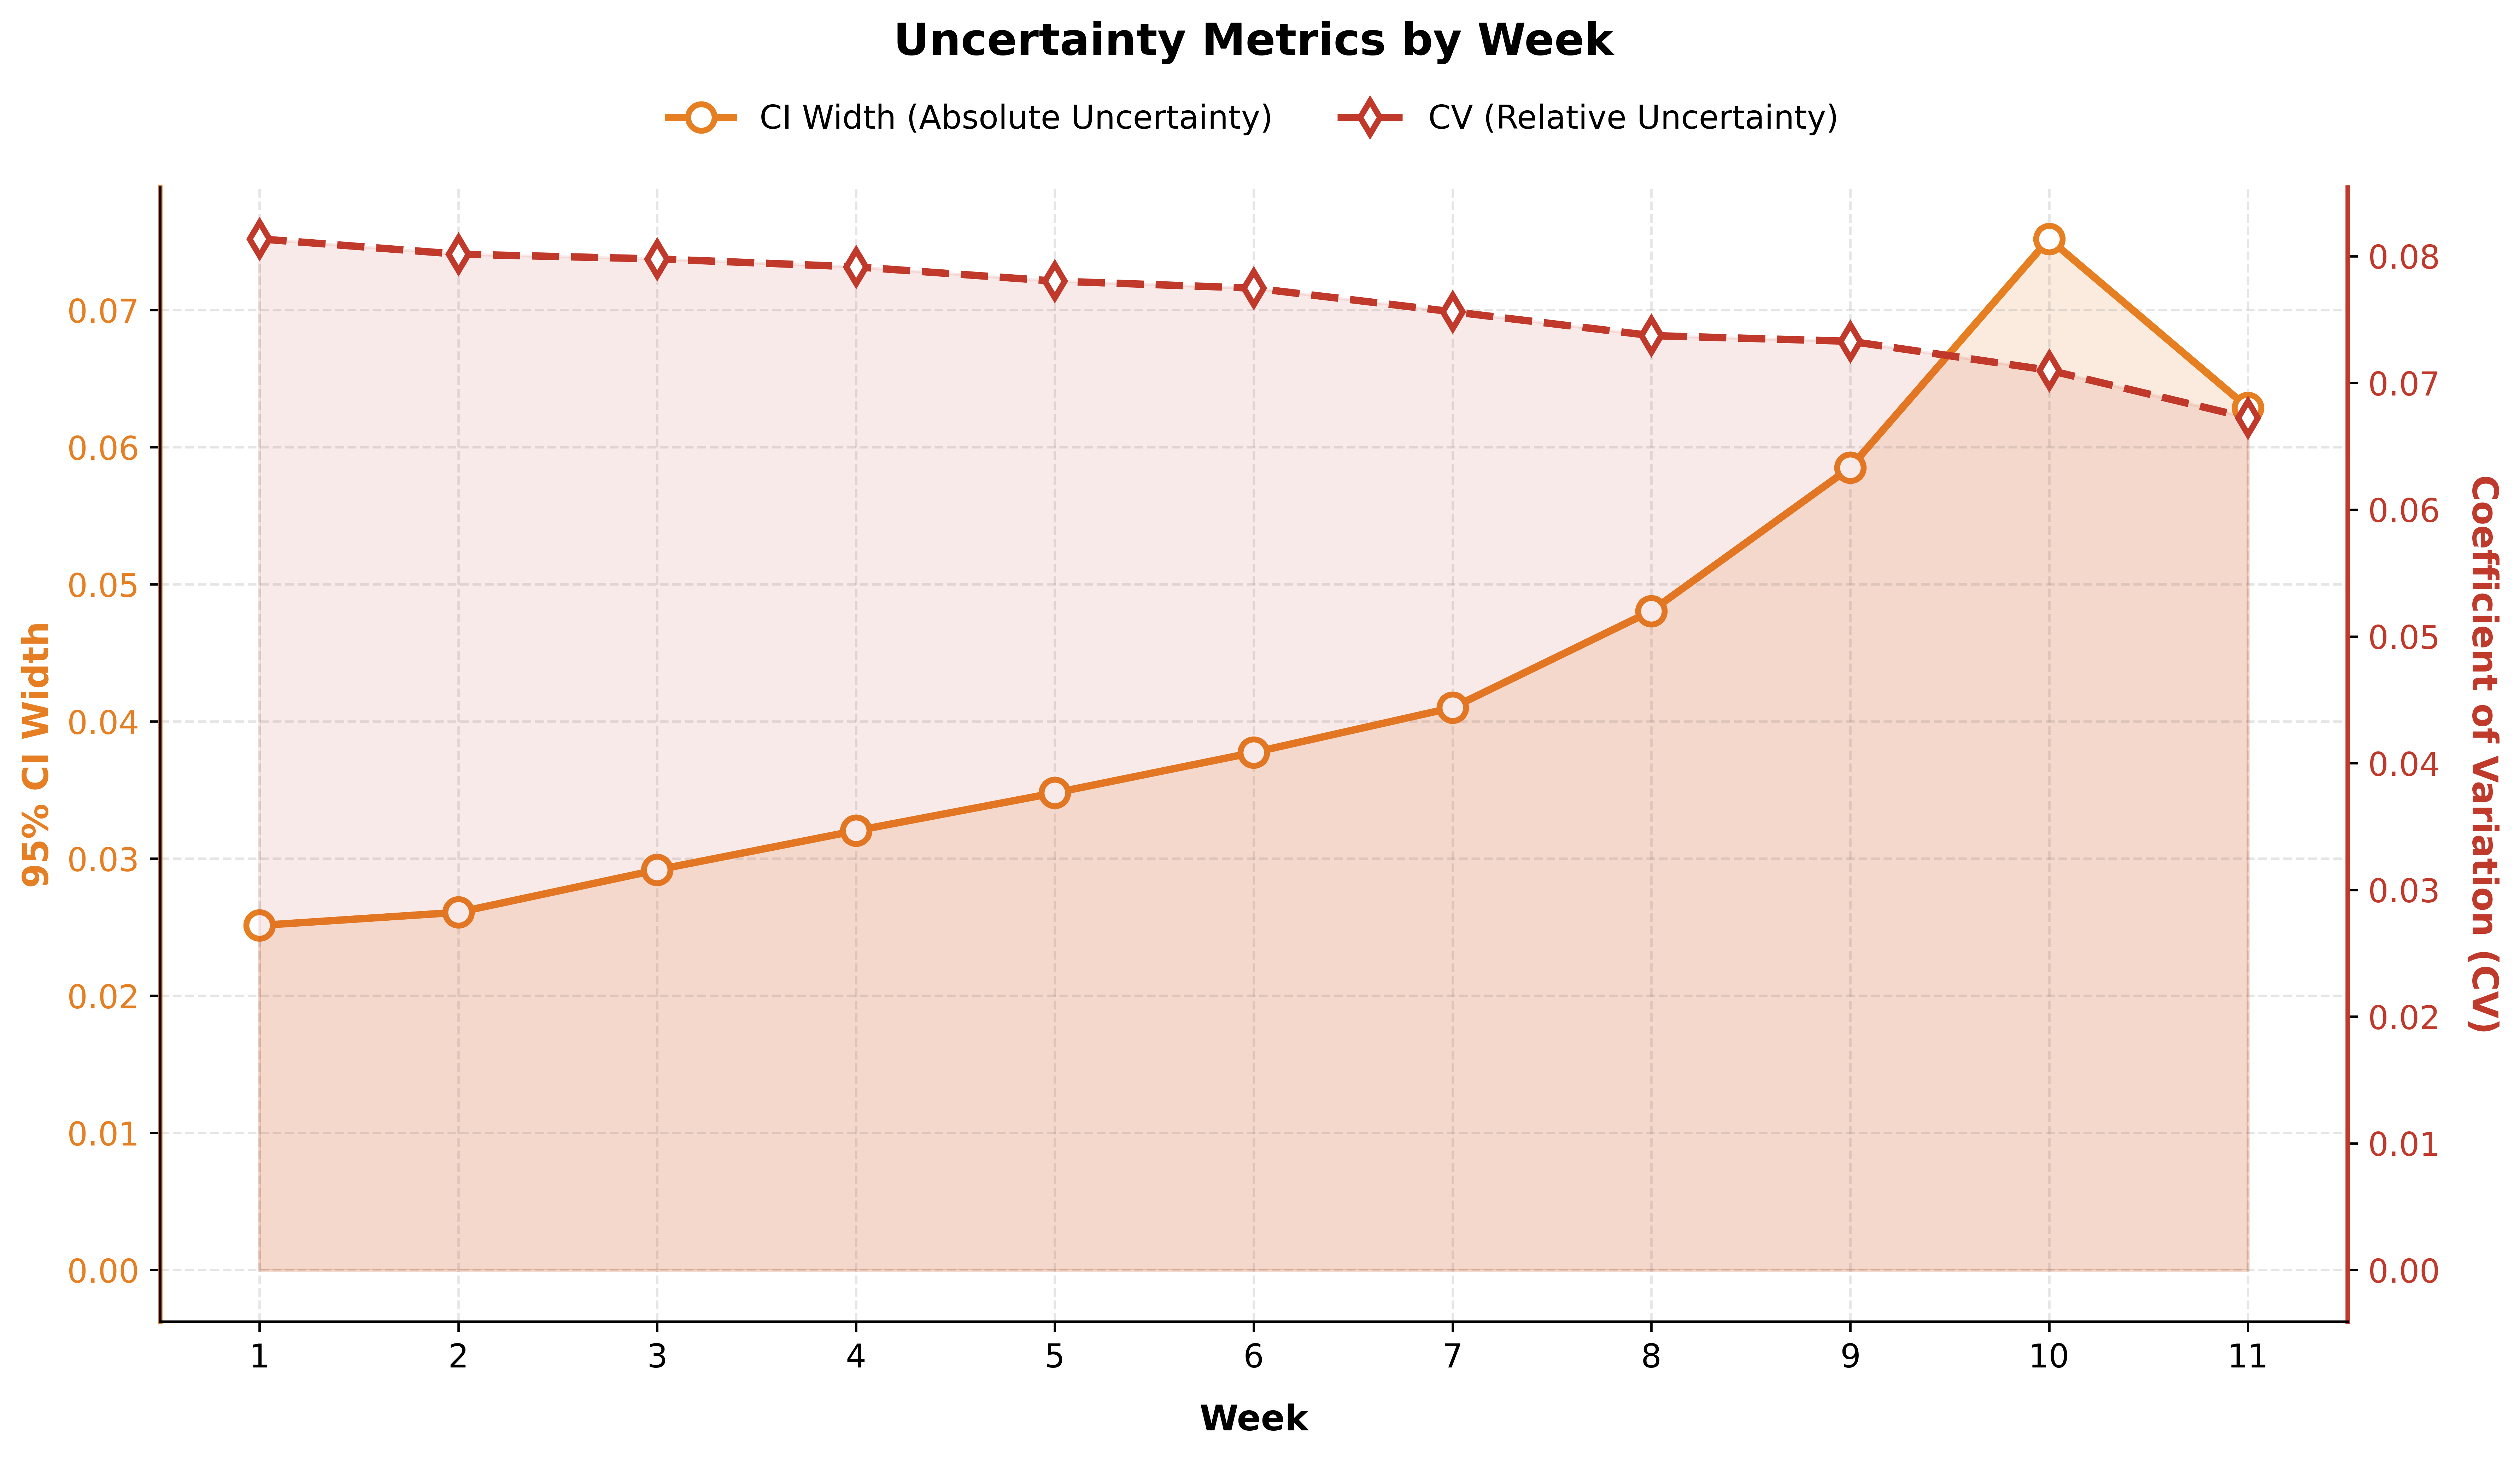
\includegraphics[width=\linewidth]{figures/T1-unv.png}
    \caption{Uncertainty Metrics by Week}
    \label{fig:t1-unv}
  \end{subfigure}
  \hfill
  \begin{subfigure}[t]{0.49\linewidth}
    \centering
    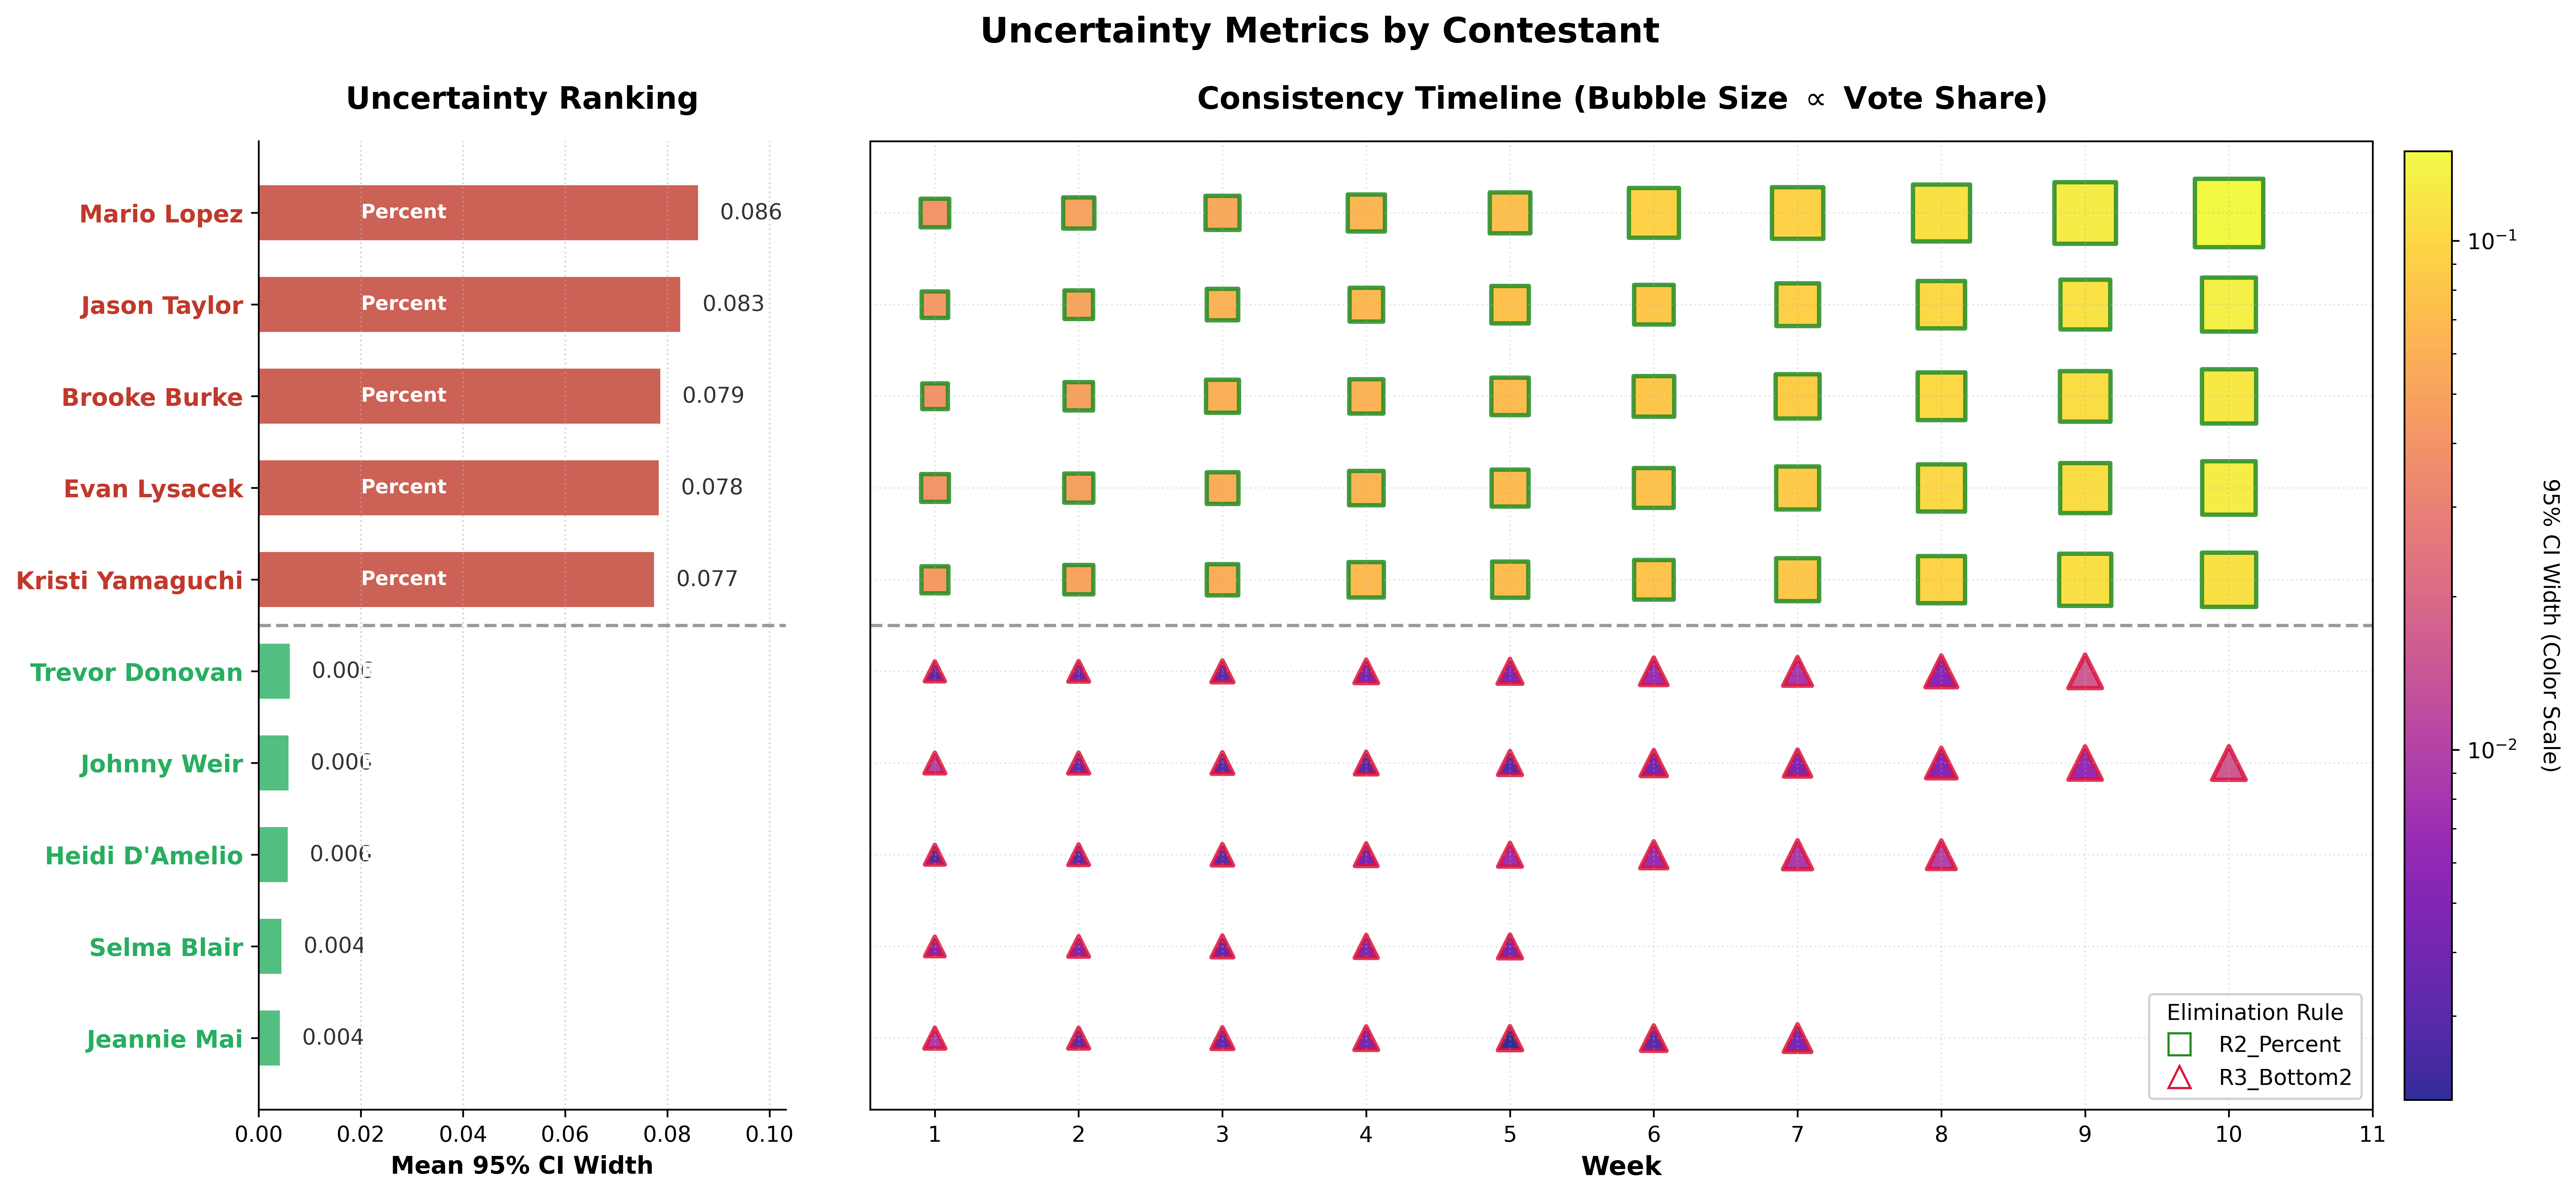
\includegraphics[width=\linewidth]{figures/T1-bubble.png}
    \caption{Uncertainty Metrics by Contestant}
    \label{fig:t1-bubble}
  \end{subfigure}
  \caption{Uncertainty Metrics by Week and Contestant}
  \label{fig:t1-uncertainty}
\end{figure}

From Figure5-a, we tracked the evolution of uncertainty across different weeks. The graph reveals that uncertainty is lower during the early stages of the season. As more contestants are eliminated, uncertainty increases. This may occur because contestants with smaller fan bases tend to be eliminated early, leaving those with larger fan bases to compete. As the competition progresses, the competition among contestants with large fan bases intensifies, leading to outcomes characterized by high uncertainty.

Additionally, from Figure5-b, we observed variations in uncertainty among different contestants. Significant differences in uncertainty levels were found between contestants. For instance, Mario Lopez had the highest mean(W) value at approximately 0.0860, while Jeannie Mai had the lowest at around 0.042—a nearly 20-fold difference. However, deeper analysis reveals that these variations in uncertainty are less tied to the contestants themselves and more influenced by the elimination rules and the week of elimination. As shown in the chart, the top 5 contestants in uncertainty rankings all followed the Percentage rule and were eliminated later, while the bottom 5 contestants in uncertainty rankings all followed the Bottom-2 rule and were eliminated earlier.

%%%%%%%%%%%%%%%%%%%%%%%%%%%%%%%%%%%%%%%%
\section{Task 2: Voting Rules Comparison, Controversy Reassessment, and Future Recommendation}
\subsection{Season-wide Rule Comparison: Rank vs. Percent}
\subsection{Agreement and Divergence}
We first reconstruct weekly fan vote shares from Problem 1 outcomes and then replay each season under both the rank-based and percentage-based rules, holding the same judge scores and estimated fan support fixed. Simulation results are summarized in Table~\ref{tab:rank-vs-pct-summary}.

\begin{table}[H]
  \centering
  \caption{Season-wide comparison between rank-based and percentage-based rules.}
  \label{tab:rank-vs-pct-summary}
  \begin{tabular}{l c}
    \toprule
    Metric & Value \\
    \midrule
    Consistent elimination weeks & \textbf{84.3\%} \\
    Spearman correlation of overall rankings & \textbf{0.786} \\
    Champion consistency rate & \textbf{47.1\%} \\
    Similarity of top-three finisher sets & \textbf{55.0\%} \\
    \bottomrule
  \end{tabular}
\end{table}

This reveals a core contradiction: minor discrepancies in overall rankings can accumulate and amplify through the elimination chain, ultimately changing the champion.

\subsubsection{Agreement in Eliminations, Divergence}

When evaluating whether scoring rules favor fan voting, we limit our analysis to scenarios where judges' and audience preferences conflict significantly. Only in such cases do the trade-offs inherent in the rule structure genuinely alter who gets eliminated.

To this end, we define a conflicting-sample set $\mathcal{H}$: each observation $(i,t)$ satisfies that the contestant ranks low in the judges' ordering but high in the fans' ordering in that week. Based on this set, we construct two complementary indices to characterize bias. The first one is \textit{Rule Bias Index (RBI)}, which measures, in a long-run average sense, the degree to which the rule protects fan-favored contestants. Let $S_{i,t}^m\in\left\{0,1\right\}$ denote whether contestant $i$ survives in week $t$ under rule $m\in\left\{\mathrm{rank},\mathrm{pct}\right\}$, then
\begin{equation}
  \mathrm{RB}\mathrm{\operatorname{I}}_{\mathrm{fan}}=\frac{1}{\left|\mathcal{H}\right|}\sum_{\left(i,t\right)\in\operatorname{H}}\left(\operatorname{S}_{i,\operatorname{t}}^{\mathrm{rank}}-\operatorname{S}_{i,\operatorname{t}}^{\mathrm{pct}}\right)
\end{equation}

We obtain ${\rm \operatorname{RBI}}_{\mathrm{fan}}=\textbf{+0.064}$, which is statistically significant. This indicates that among samples where judges' and fans' preferences conflict, the rank-based rule is, on average, less likely to eliminate fan-favored contestants. To reveal the trade-offs when the two rules truly diverge, we define a second index, \textit{Flip-to-Fan Index (FTF)}. Focusing on the set of weeks $\mathcal{K}$ in which the rules disagree, we assess whether the contestant eliminated by each rule is less aligned with fans' preference, i.e.,
\begin{equation}
  \mathrm{FTF}=\frac{1}{\left|\mathcal{K}\right|}\sum_{t\in\mathcal{K}} d\left(t\right)
\end{equation}

Here $d\left(t\right)\in\left\{-1,+1\right\}$ indicates the direction of bias in week $t$, and a positive value means that the eliminated contestant is ranked lower by fans. Among 63 disagreement weeks, the rank-based rule aligns better with fan preference in 30 weeks, while the percentage-based rule does so in 33 weeks, yielding $\mathrm{FTF}=\textbf{-0.0476}$. This suggests that when the two rules make different choices, the percentage-based rule tends to be more consistent with audience preference by eliminating contestants who are relatively less supported by fans.

Further analysis shows that rule bias does not simply benefit all popular contestants. Define the within-week controversy ${\rm Discrepancy}_{i,t}$ as the difference between contestant $i$'s fan vote share and judges' score share in week $t$ (both normalized). 

The results show that when we restrict attention to the ``most popular of the week'' samples alone, $\mathrm{FTF}=\textbf{-0.017}$ and is not statistically significant; only in the intersection region of ``high popularity'' and ``high discrepancy'' does $\mathrm{FTF}$ become significantly \textbf{positive}. In other words, the effect of rule differences mainly operates at moments when judges' and audience preferences conflict most severely, and it propagates through the elimination chain to ultimately change the champion, which corroborates our earlier conclusion.
\subsection{Controversial Cases Identification}

Building on the measurement of ${\rm Discrepancy}_{i,t}$ in Section 4.1, we further construct two season-level indicators, intensity and persistence, to systematically identify the ``controversial contestants''. Intensity reflects the average magnitude of disagreement between judges' evaluations and audience preferences for a contestant, while persistence measures how long the contestant remains in a ``high-discrepancy'' state.

Let $\mathcal{T}_{i,s}$ denote the set of weeks in which contestant $i$ actually competes in season $s$, and let $T_{i,s}$ be the number of competing weeks. Let $I_{i,t}$ denote the magnitude of disagreement between judges and fans in week $t$, and let $H_{i,t}\in0,1$ be an indicator variable of whether week $t$ is a ``high-discrepancy week.'' We then define
\begin{equation}
\mathrm{Intensit}\mathrm{\operatorname{y}}_{\mathrm{i,s}}\;=\;\frac{1}{T_{i,s}}\sum_{t\in\mathcal{T}_{\mathcal{i},\mathcal{s}}} I_{i,t}
\end{equation}
\begin{equation}
\mathrm{Persistenc}\mathrm{\operatorname{e}}_{\mathrm{i,s}}\;=\;\frac{1}{T_{i,s}}\sum_{t\in\mathcal{T}_{\mathcal{i},\mathcal{s}}} H_{i,t}
\end{equation}
We employed the intensity-persistence two-quadrant method for identification: athletes scoring above the set threshold in both dimensions were defined as high-controversy athletes. Based on this criterion, a total of 72 athletes meeting the standard were identified. The core of this method lies in distinguishing between “incidental” and “structural” controversies: the latter requires disagreements to be not only intense but also recurring. The calculated metrics for four representative cases are as Table~\ref{tab:typical controversy cases}. 

\begin{table}[htbp]
  \centering
  \caption{Controversy metrics (Intensity, Persistence) for selected contestants}
  \label{tab:typical controversy cases}
  \begin{tabular}{lcc}
    \toprule
    Contestant & Intensity & Persistence \\
    \midrule
    Jerry Rice & 1.001 & 0.800 \\
    Bristol Palin & 1.397 & 0.850 \\
    Bobby Bones & 1.409 & 1.000 \\
    Billy Ray Cyrus & 0.397 & 0.150 \\
    \bottomrule
  \end{tabular}
\end{table}

It's worth noting that Billy Ray Cyrus did not generate sustained “structural controversy” under our analytical framework, so his race results did not have the same structural impact on championship outcomes as those of Jerry Rice or Bobby Bones.
We employ the direction of disagreement to focus on specific points of contention: based on the magnitude and polarity of the mean ${\rm Discrepancy}_{i,t}$, contestants are categorized into three groups: fan-favored, judge-favored, and neutral (see Fig.~\ref{fig:q2_two_panels:a}).

\begin{figure}[H]
  \centering
  \begin{subfigure}[t]{0.49\linewidth}
    \centering
    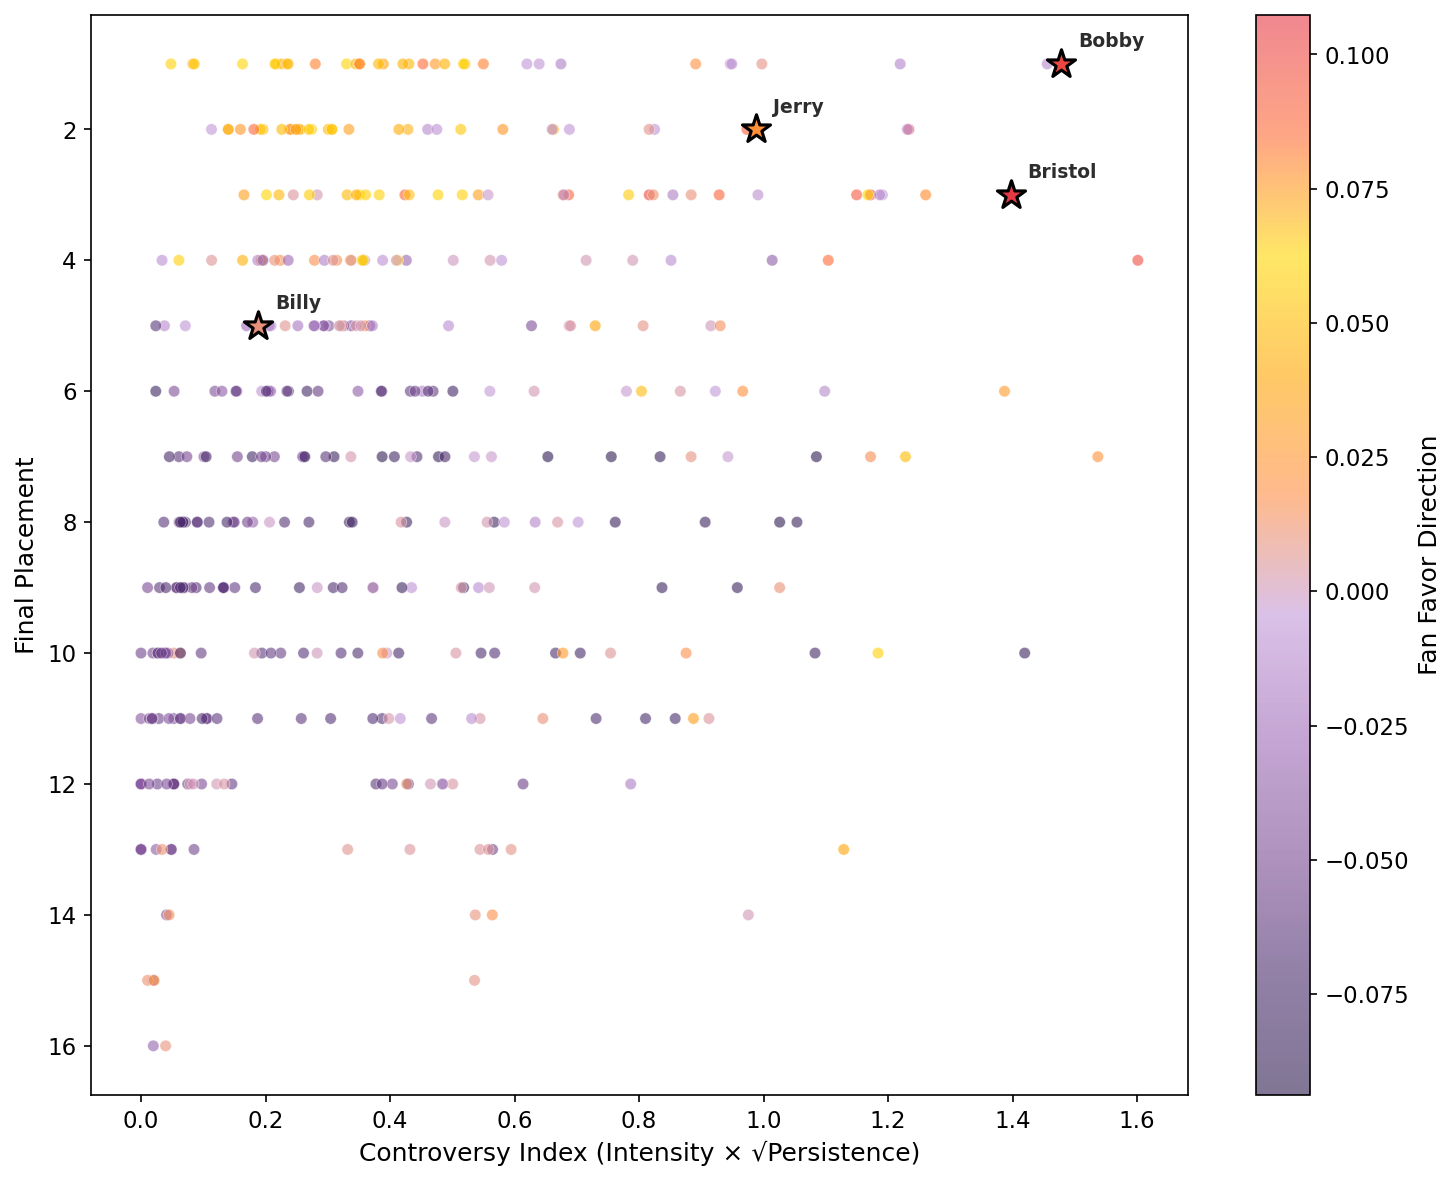
\includegraphics[width=\linewidth]{q2_controversy_alpine_glow}
    \caption{Controversy Index vs. Final Placement with Favor Direction}
    \label{fig:q2_two_panels:a}
  \end{subfigure}\hfill
  \begin{subfigure}[t]{0.49\linewidth}
    \centering
    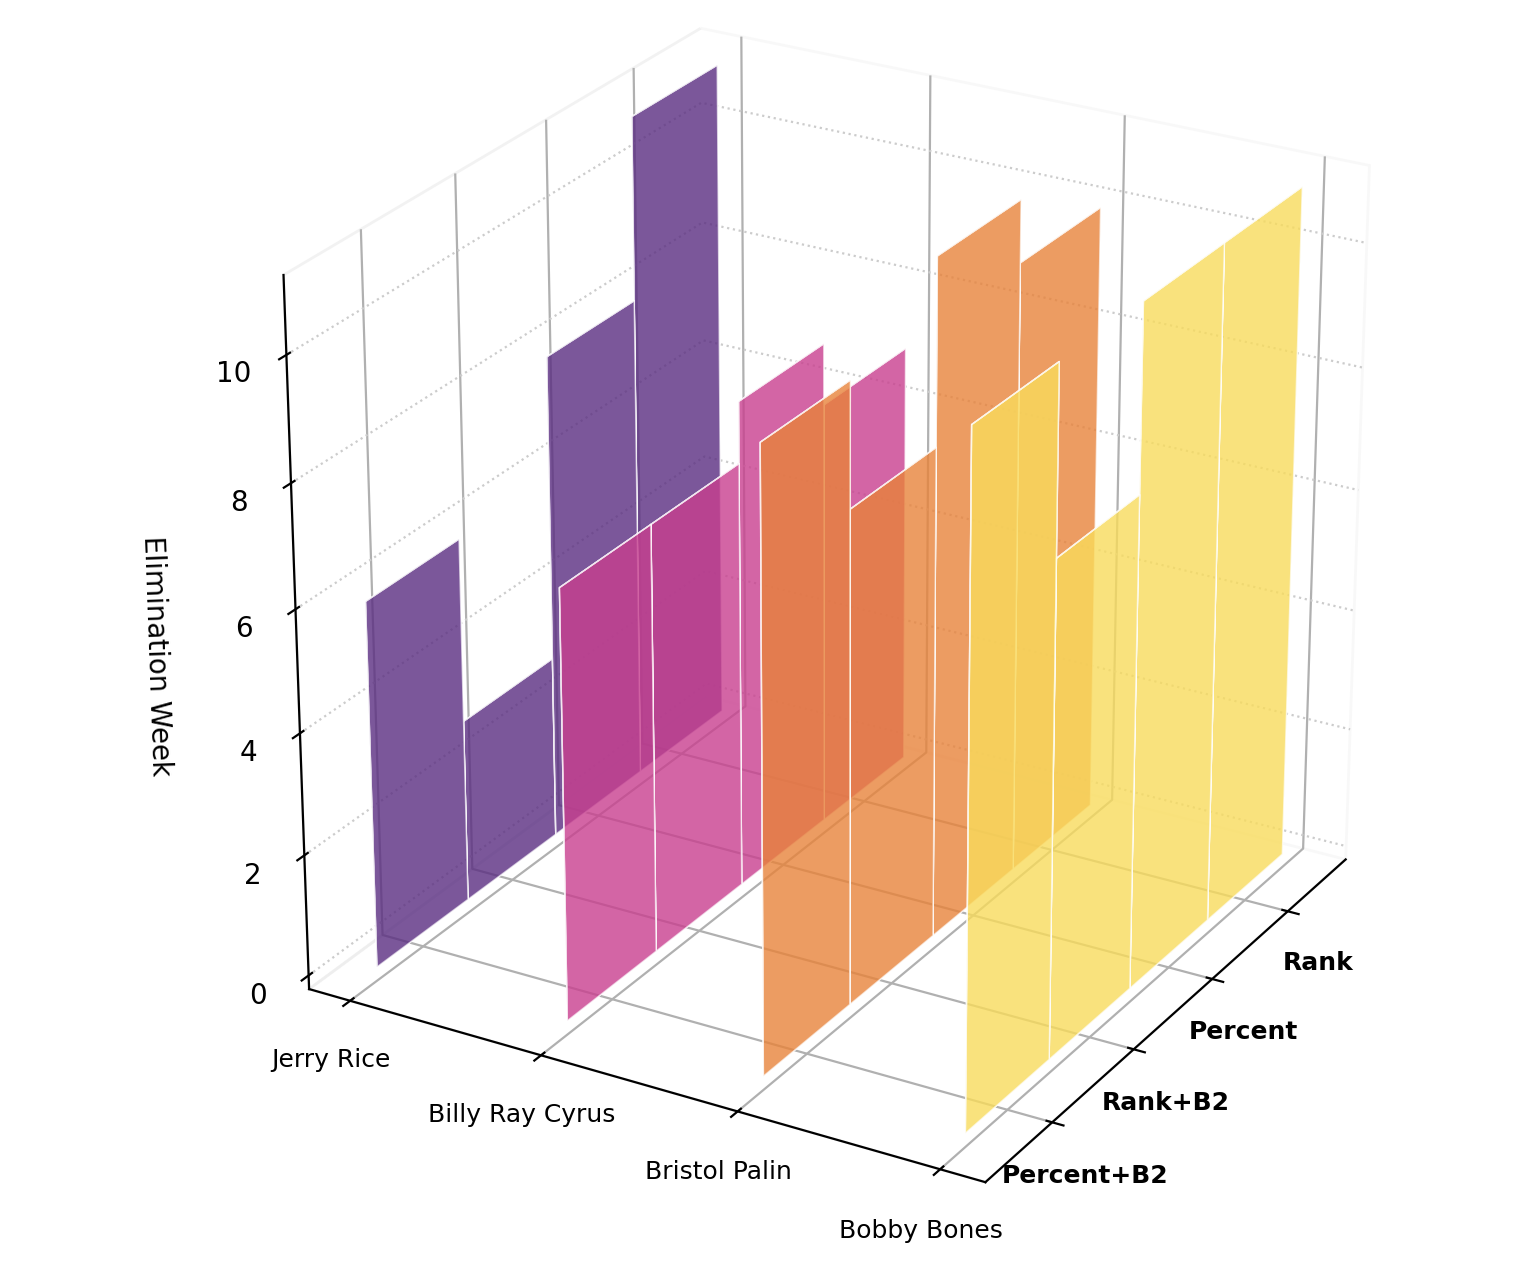
\includegraphics[width=\linewidth]{q2_3d}
    \caption{Survival Periods of Typical Cases Under Different Rules}
    \label{fig:q2_two_panels:b}
  \end{subfigure}
  \caption{Key visual diagnostics for Q2: controversy outcomes and rule-dependent survival patterns.}
  \label{fig:q2_two_panels}
\end{figure}

After identification, we conducted counterfactual comparisons for each season. The results indicate that rule variations primarily impacted highly contested contestants during a few critical weeks, consistent with the mechanism described in Section 4.1. Taking the four representative contestants listed as examples, the simulation results are shown in Table~\ref{tab:loophole1_diag}. 
\begin{table}[htbp]
\centering
\small
\setlength{\tabcolsep}{4pt}
\renewcommand{\arraystretch}{1.15}
\caption{Placement Shifts and Pivotal Weeks}
\label{tab:loophole1_diag}
\begin{tabular}{l c c c c c p{2.4cm} p{2.4cm}}
\toprule
 &  & \multicolumn{4}{c}{\textbf{Placement under Each Rule}} & \multicolumn{2}{c}{\textbf{Pivotal Detrimental Weeks}} \\
\cmidrule(lr){3-6}\cmidrule(lr){7-8}
\textbf{Contestant} & \textbf{Actual} 
& \textbf{Rank} & \textbf{Percent} & \textbf{Rank+B2} & \textbf{Percent+B2}
& \textbf{Rank} & \textbf{Percent} \\
\midrule
Jerry Rice        
& 2 
& $2\,(+0)$ & $\textbf{5\,(+3})$ & $3\,(+1)$ & $3\,(+1)$ 
& -- & W8 \\

Billy Ray Cyrus   
& 5 
& $\textbf{8\,(+3)}$ & $6\,(+1)$ & $8\,(+3)$ & $7\,(+2)$
& W7 & -- \\

Bristol Palin     
& 3 
& $\textbf{4\,(+1)}$ & $2\,(-1)$ & $6\,(+3)$ & $5\,(+2)$
& W10 & -- \\

Bobby Bones       
& 1 
& $\textit{5\,(+4)}$ & $\textit{5\,(+4)}$ & $7\,(+6)$ & $5\,(+4)$
& -- & -- \\
\bottomrule
\end{tabular}
\end{table}

Extending the analysis to highly contested groups reveals that rule variations similarly exhibit a concentrated elimination pattern: highly contested contestants survived an average of 6.7 weeks under rank-based rule and 6.4 weeks under percent-based rule. When Judge's Save was introduced, average survival periods decreased to 6.4 and 6.3 weeks respectively, indicating that this mechanism systematically reduces survival space for contested contestants. 

This conclusion remains robust to variations in judge decision uncertainty: simulations under deterministic (eliminating the contestant with the lower total score) and random decision scenarios showed only a 0.45-week difference in average survival. This indicates that the directional finding that “Judge's Save tilts outcomes toward the judges” does not depend on any specific decision-making assumption.


%%%%%%%%%%%%%%%%%%%%%%%%%%%%%%%%%%%%%%%%
\section{Task 3: Structural Comparison of Judges’ Scoring and Fans’ Voting Preferences}
\subsection{Overview}
Data analysis reveals significant temporal trends in both judge scores and fan votes as the competition progresses through weekly rounds. Judge scores show a marked increase in later stages compared to earlier ones, while fan vote distribution shifts from initial concentration to greater dispersion later on. This phenomenon largely stems from overall improvements driven by the show's scoring conventions and performers' growing proficiency. Additionally, although celebrities and dancers form fixed partnerships within each season, the same dancers partner with different celebrities across multiple seasons, creating cross-seasonal correlations in the overall data. Simultaneously, Task~1 demonstrated that a single celebrity's performance across different weeks exhibits high correlation. Failing to account for these three structural characteristics would conflate dancer ability with competition progression and celebrity popularity with dancer skill, rendering results incomparable. Conventional linear MixedLM or regression models, which use linear week variables to capture temporal trends, would erroneously attribute the nonlinear scoring improvement driven by the competition's progression to celebrity or dancer ability, leading to systematic bias in random effect estimates. We developed a model called ``Hierarchical Semi-Parametric Variance Decomposition'' (HSVD) to decompose performance variations into time effects, celebrity effects, and dancer effects under both evaluation systems.

\begin{figure}[H]
  \centering
  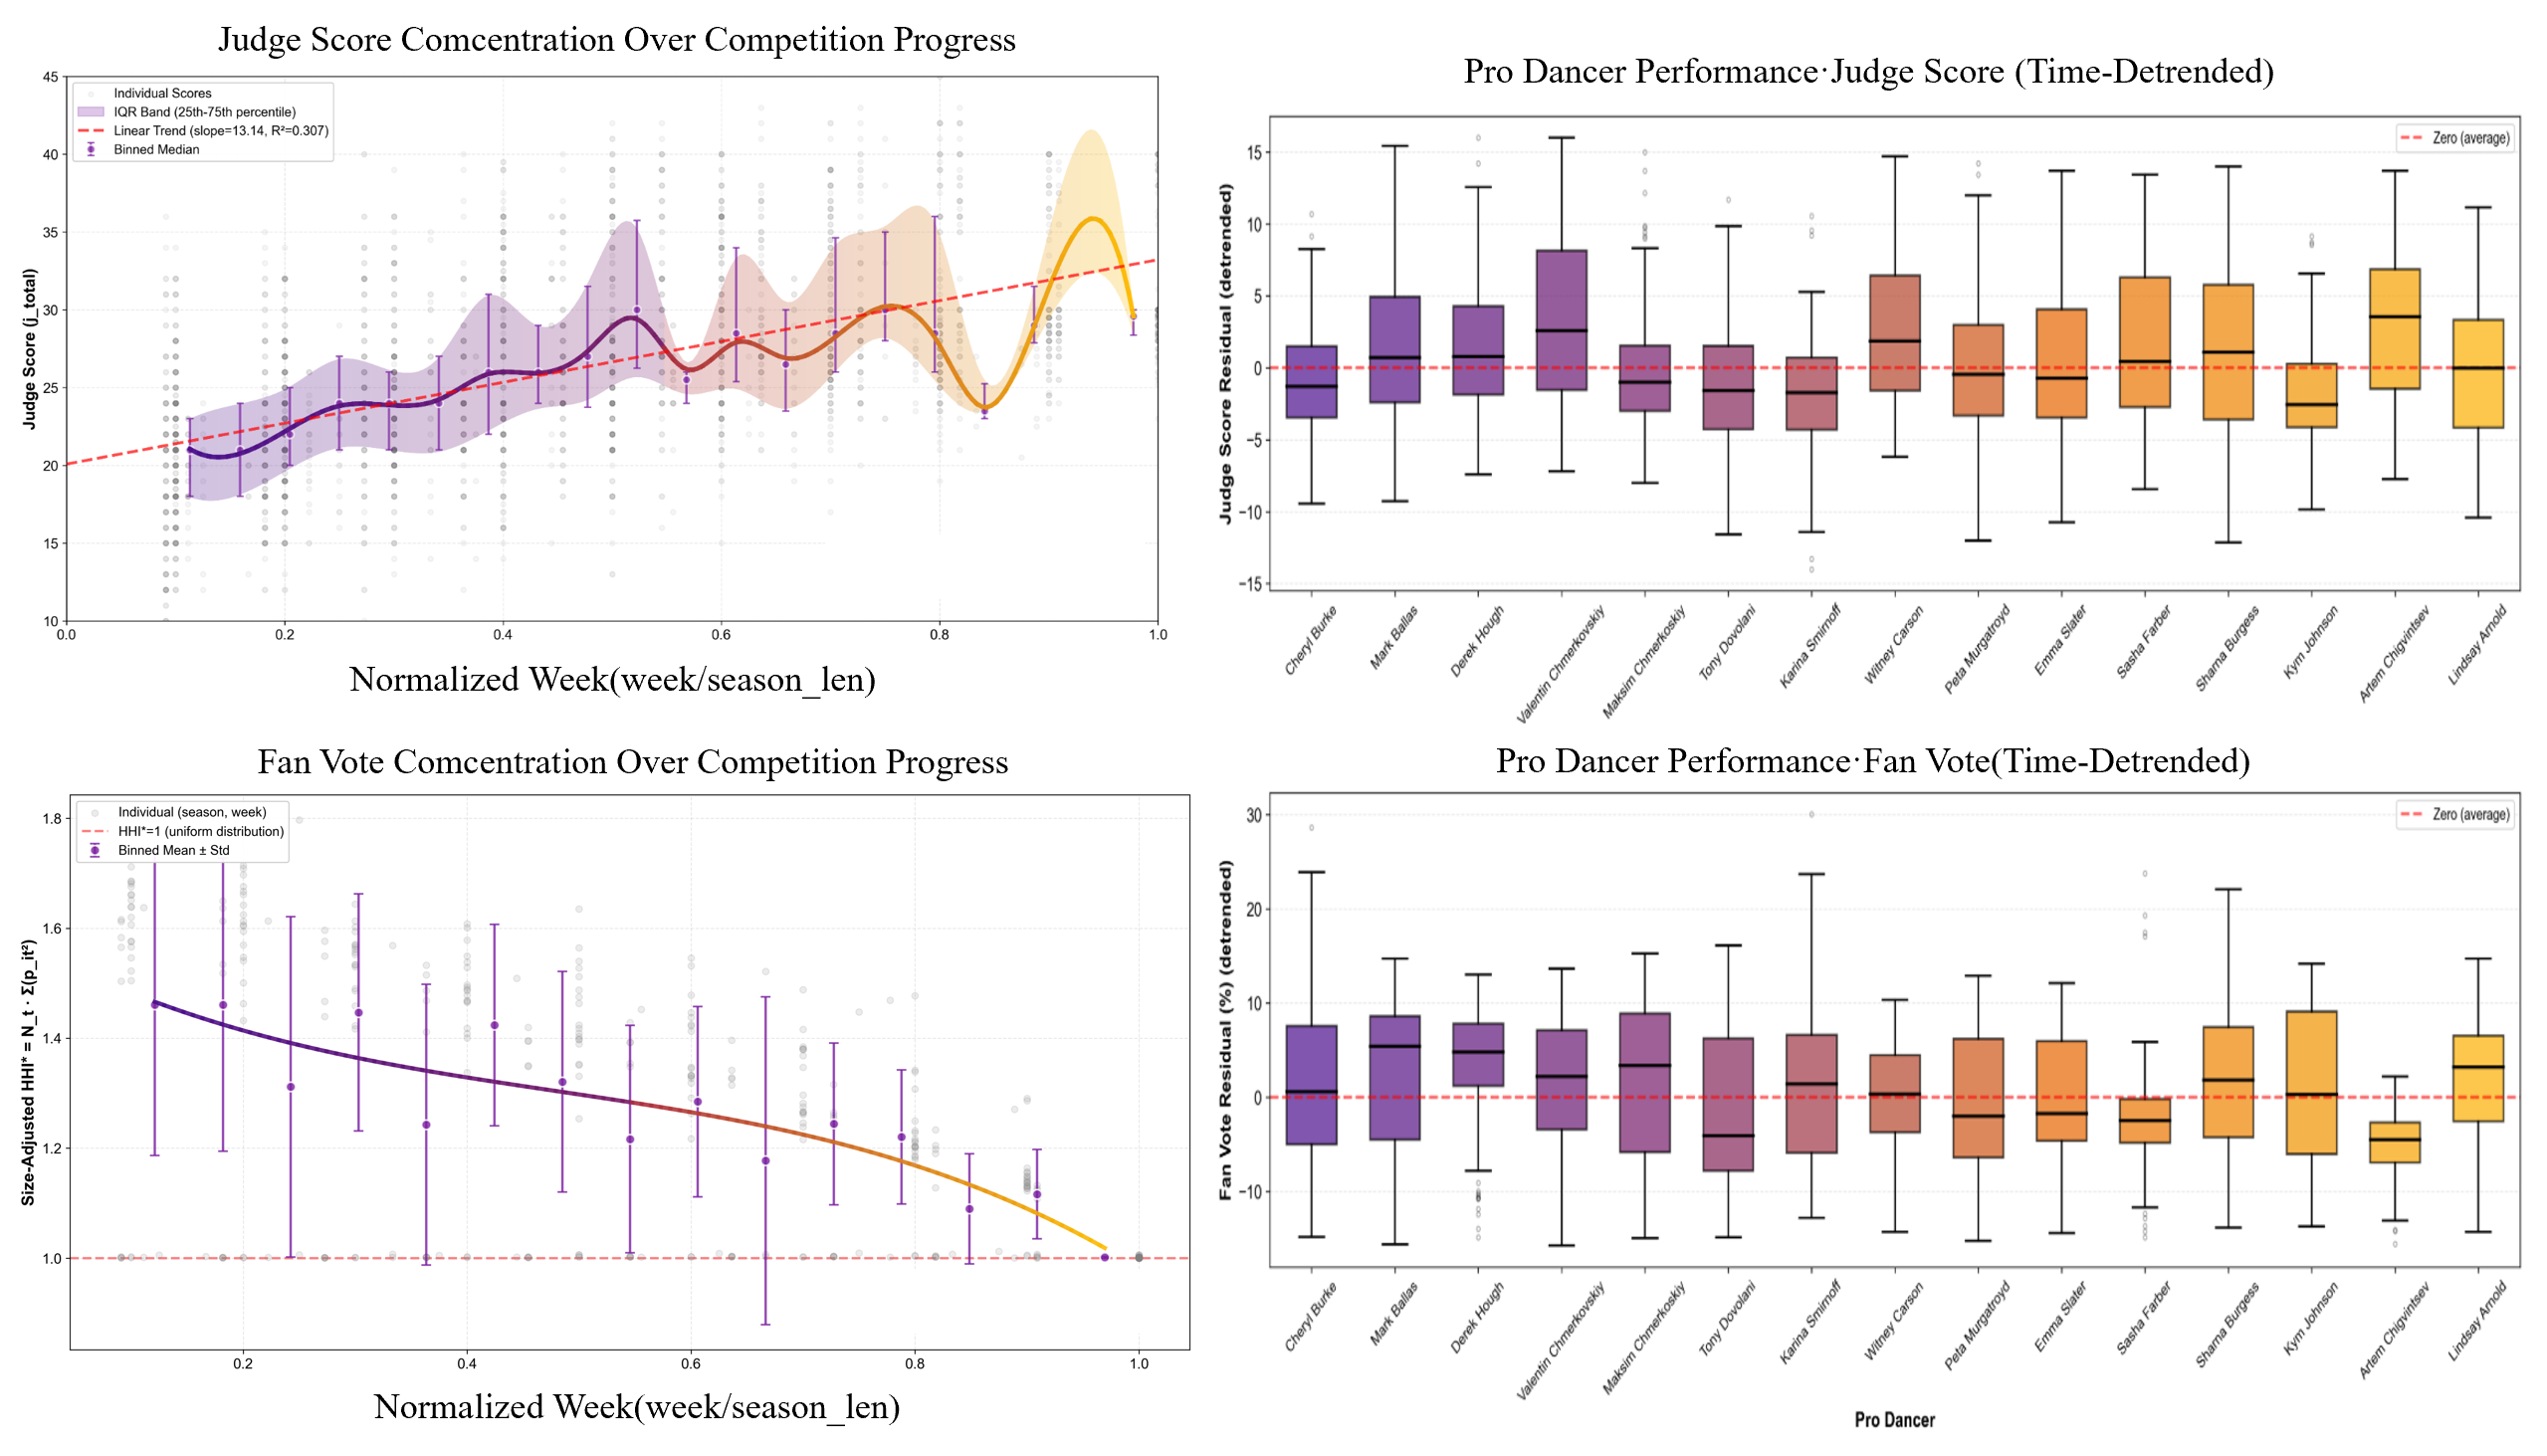
\includegraphics[width=0.92\linewidth]{T3_1}
  \caption{Temporal Trends and De-trended Pro-Dancer Effects in Judges and Fan Evaluations}
  \label{fig:t3-1}
\end{figure}

\subsection{Structural Interpretation Under the HSVD Framework}
Due to variations in the number of weeks across different seasons, using the raw week variable directly would introduce season length differences into the model, interfering with the depiction of temporal trends. To ensure comparability of time effects across seasons, we normalize the week variable, defining it as the player's relative progress within their respective season.
\[
  \tilde{w}_{it}=\frac{\text{week}_{it}}{\text{season\_len}_s}
\]
Regarding the weekly performance of celebrity contestants, we propose it comprises five components: the time effect driven by the progression of the competition schedule, unobservable random contributions from both celebrity contestants and professional dancers, observable attributes of both parties, and random disturbance terms. Building upon this, the HSVD framework further decomposes the unobservable structural variance into three components: time effect, celebrity random effect, and professional dancer random effect. By constructing two symmetric models with identical structures but swapped dependent variables, we ensure strict comparability between the two evaluation systems. This allows us to identify differences in the roles of celebrities and dancers across these distinct evaluation frameworks.Throughout the competition, both judges' scores and fan voting patterns exhibited nonlinear changes as the tournament progressed. Therefore, we employed a semi-parametric smoothing approach based on spline functions to capture the stage-specific effects of the tournament schedule, thereby eliminating confounding factors introduced by temporal trends.
\[
  j_{it}
  =
  \alpha^{J}
  + s^{J}(\tilde{w}_{it})
  + \beta_1^{J} \text{Age}_i
  + \beta_2^{J} \text{Age}_i^2
  + \beta_3^{J} \text{Exposure}_i
  + \beta_4^{J} \text{Exposure}_i^2
  + \mathbf{Z}_i^\top \boldsymbol{\gamma}^{J}
  + u_i
  + v_{p(i)}
  + \varepsilon_{it}^{J}
\]

\[
  \text{logit}(p_{it}^{V})
  =
  \alpha^{F}
  + s^{F}(\tilde{w}_{it})
  + \beta_1^{F} \text{Age}_i
  + \beta_2^{F} \text{Age}_i^2
  + \beta_3^{F} \text{Exposure}_i
  + \beta_4^{F} \text{Exposure}_i^2
  + \mathbf{Z}_i^\top \boldsymbol{\gamma}^{F}
  + u_i
  + v_{p(i)}
  + \varepsilon_{it}^{F}
\]

\[
  \text{logit}(p) = \ln\left(\frac{p}{1-p}\right)
\]

\[
  u_i \sim \mathcal{N}(0,\sigma_c^2), \qquad
  v_{p(i)} \sim \mathcal{N}(0,\sigma_d^2)
\]

\subsection{Analysis Results}
\subsubsection{The Influence of Dancer and Celebrity Characteristics on Competition Performance}
\begin{figure}[H]
  \centering
  \begin{subfigure}[t]{0.49\linewidth}
    \centering
    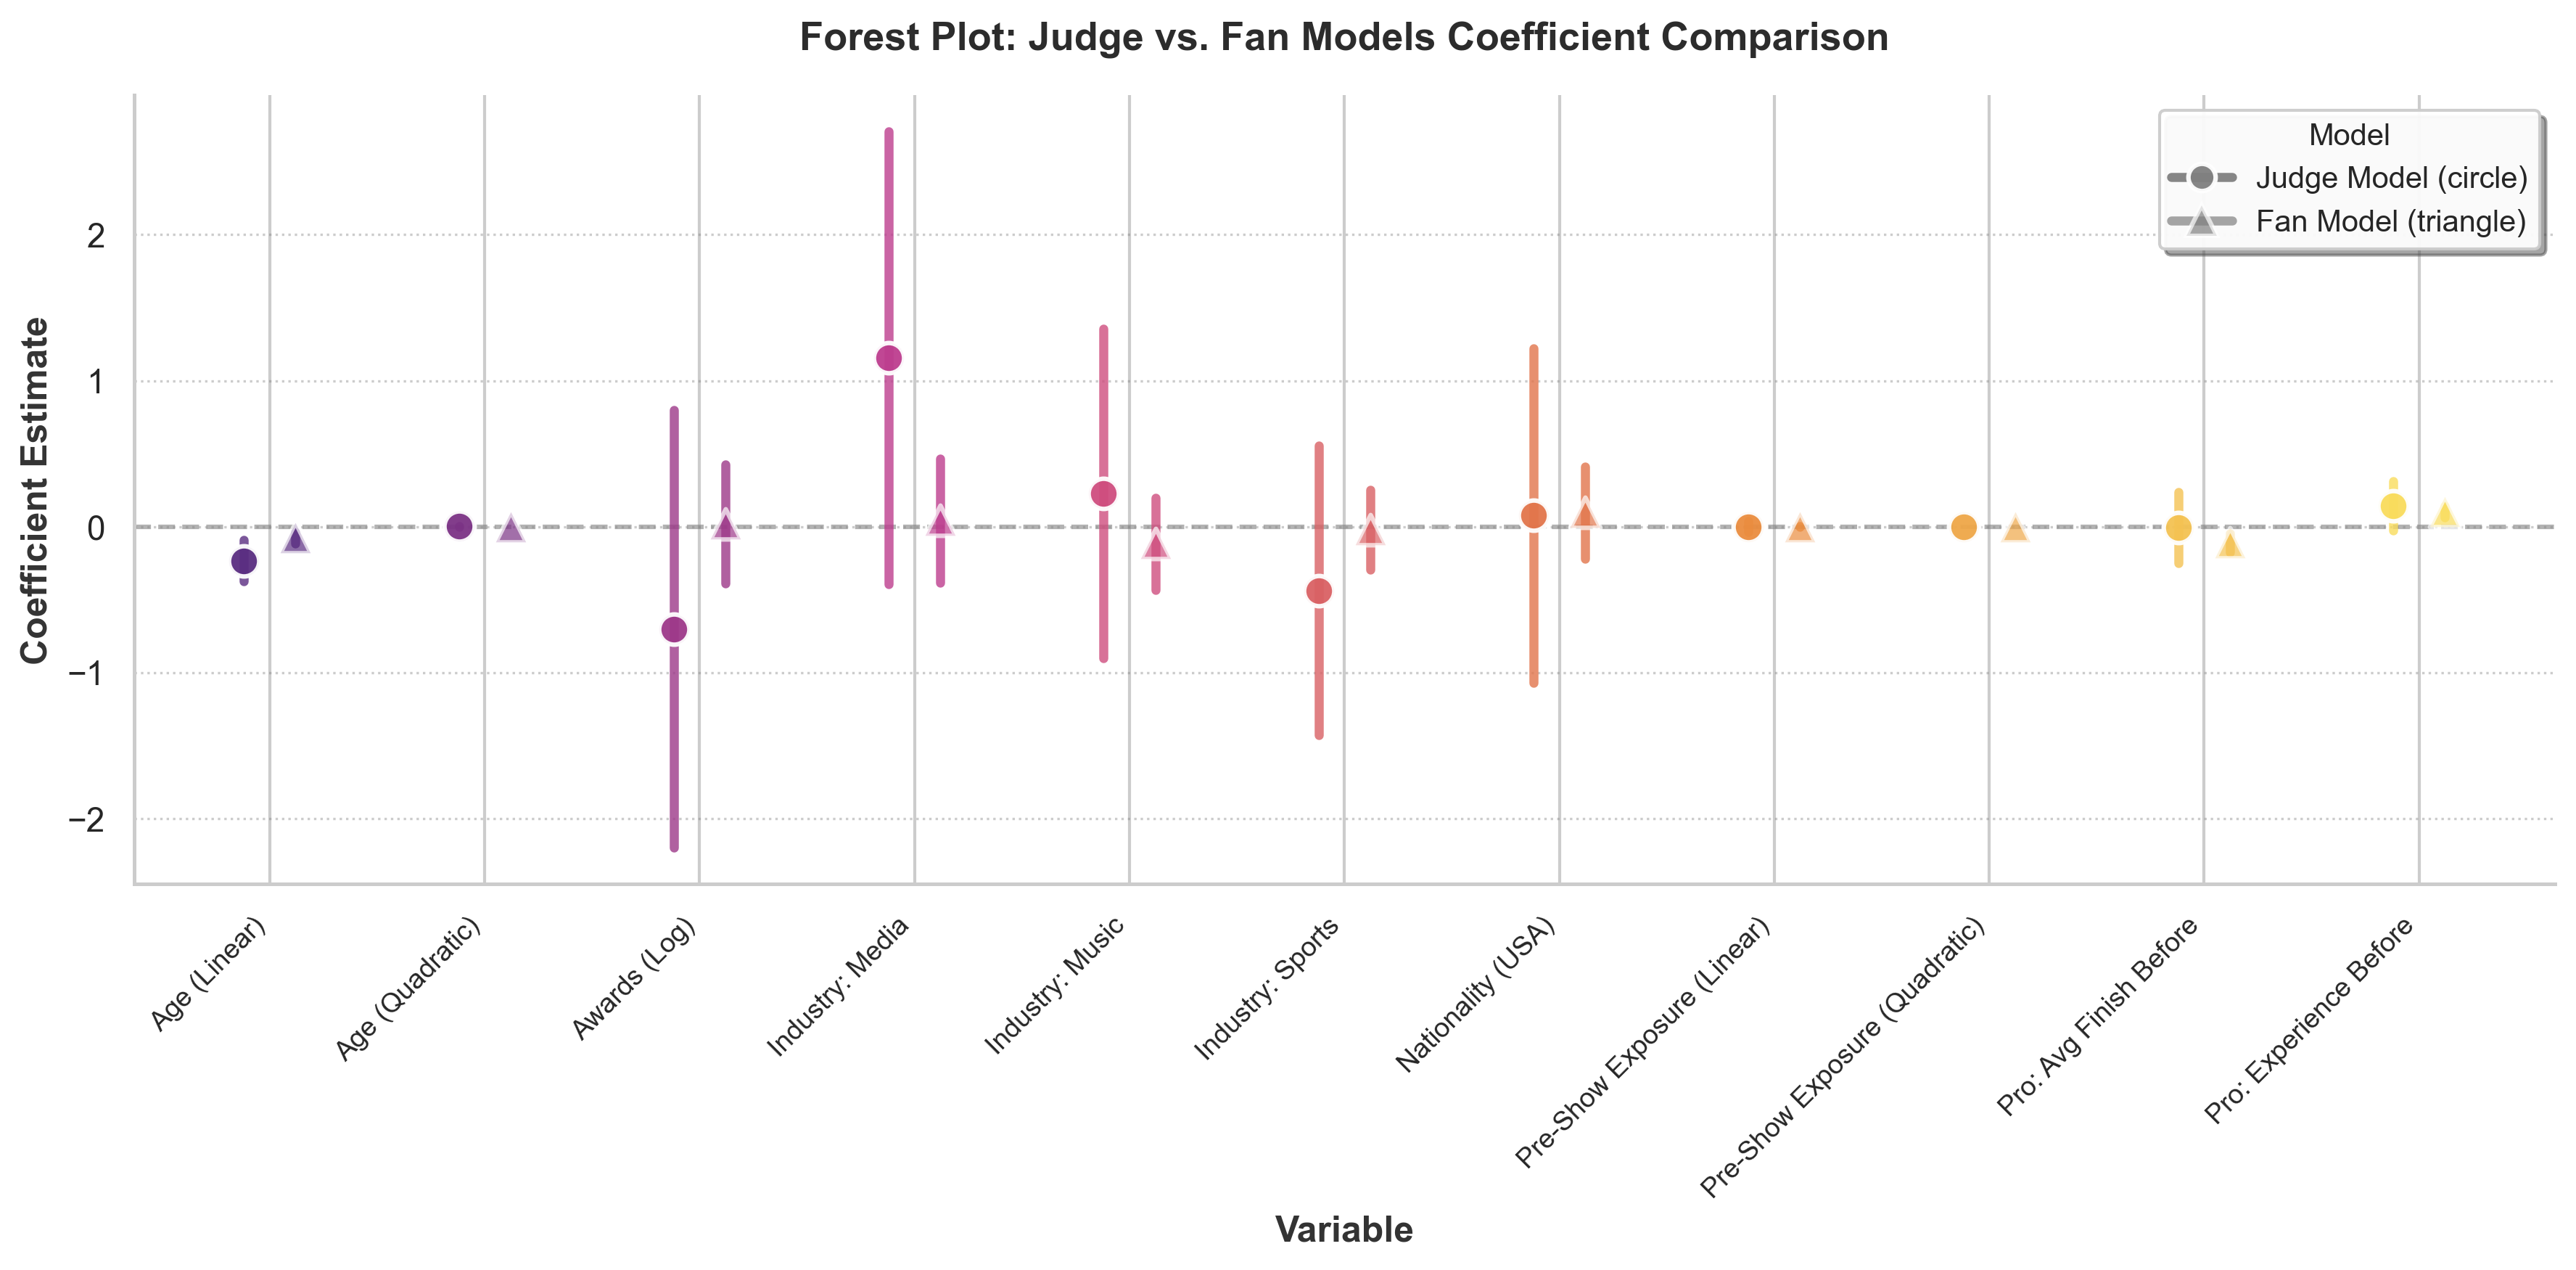
\includegraphics[width=\linewidth]{figures/T3_3.png}
    \caption{Dominant Trait Comparison Chart}
    \label{fig:t3-3a}
  \end{subfigure}
  \hfill
  \begin{subfigure}[t]{0.49\linewidth}
    \centering
    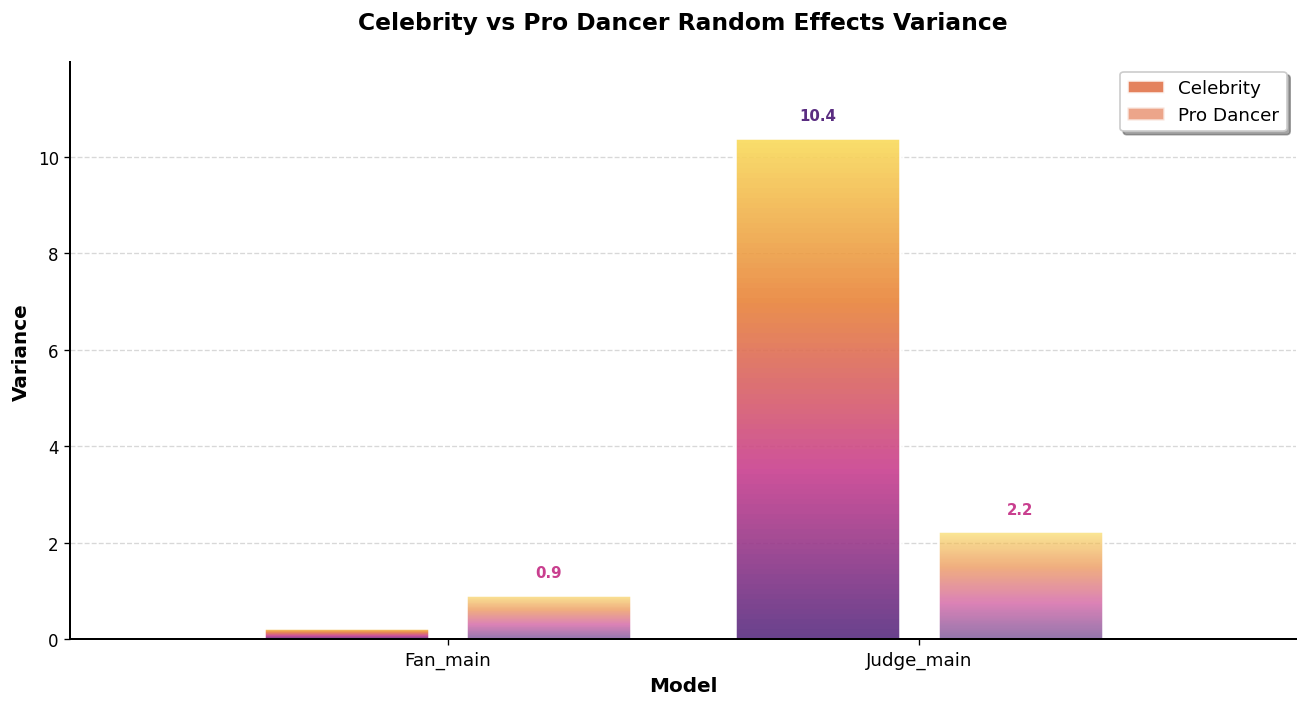
\includegraphics[width=\linewidth]{figures/T3_4.png}
    \caption{Random Effects Variance Bar Chart}
    \label{fig:t3-4}
  \end{subfigure}
  \caption{Judge vs. Fan: Coefficient Comparison of Celebrity and Pro-Dancer Features}
  \label{fig:t3-3}
\end{figure}

According to the results, competition performance is jointly influenced by the explicit attributes and implicit traits (random effects) of celebrities and dancers. For celebrities, age and pre-competition exposure are highly significant factors. Pre-competition exposure exhibits a pronounced inverted U-shaped relationship with scores, with a quadratic coefficient of approximately $-0.65$ ($p < 0.001$). This demonstrates the effectiveness of moderate promotion while highlighting that excessive marketing can lead to aesthetic fatigue. Age exhibits a pronounced negative trend, with both judges and fans demonstrating a preference for younger contestants. Industry background influences scoring differentially: media industry background yields a significant positive coefficient of approximately $+1.1$ in the judge model, while sports industry background shows a significant negative impact of approximately $-0.5$. This indicates judges hold athletes with superior physical attributes to higher standards, resulting in stricter scoring. In the fan model, a music industry background shows a slightly negative effect. Regarding contestants' award histories, while ``whether awarded'' exhibits a positive pull of $+1.12$ in the judge model, its $p$-value of $0.25$ fails to reach significance. This indicates past honors serve as a bonus but are not a core driver. Additionally, the significance of being a U.S. native contestant is extremely low ($p = 0.89$), confirming the program's fairness regarding nationality. For dancers, their resumes are crucial in determining fan votes. Each additional championship win by a dancer significantly increases their partner's fan vote Logit value by an average of $0.507$ units. Furthermore, dancers' random effects significantly impact competition outcomes, with extremely high variance in both models, quantifying the vast differences in choreography skills and teaching charisma among dancers.

\subsubsection{Consistency and Differences Between the Two Evaluation Systems}
Both scoring systems demonstrate that younger contestants hold an advantage in competition, while also confirming the nonlinear relationship between pre-competition exposure and scores, with both systems exhibiting a significantly negative quadratic coefficient. Nationality proves insignificant in both models, indicating that contestants' U.S. origin does not constitute a significant bonus or penalty under this evaluation framework. However, beneath this apparent consistency, the two systems reveal distinct characteristics in value judgment and variance allocation.

\noindent From the judges' perspective, the evaluation focus is highly concentrated on the celebrity's personal traits, with their individual random variance far exceeding that of the dancers. This reflects the judges' emphasis on the celebrity's dance talent and expressive ability. From the fans' perspective, the random variance of professional dancers dominates overwhelmingly, far exceeding that of individual celebrities. This indicates that in fan evaluations, the stage performance influenced by ``who the partner is'' often overshadows the celebrity's own performance. Simultaneously, fans are highly sensitive to dancers' past experiences. Judges, however, place greater emphasis on the technical proficiency demonstrated during the live performance. Furthermore, as mentioned earlier, both fans and judges exhibit varying degrees of differentiated perceptions across different industries.

%%%%%%%%%%%%%%%%%%%%%%%%%%%%%%%%%%%%%%%%
\section{Results}
\subsection{Main quantitative results}
\subsubsection{Result table}
\begin{table}[H]
  \centering
  \caption{Illustrative results table (replace with your real numbers).}
  \label{tab:results}
  \begin{tabular}{lcc}
    \toprule
    Method & Primary Score $\uparrow$ & Constraint Violation $\downarrow$ \\
    \midrule
    Baseline heuristic & 0.71 & 2.5\% \\
    Proposed framework & 0.80 & 0.8\% \\
    \bottomrule
  \end{tabular}
\end{table}

\subsubsection{Interpretation}
The proposed approach improves the primary score while reducing violations, indicating that the optimization layer effectively
translates predictive estimates into feasible decisions.

%%%%%%%%%%%%%%%%%%%%%%%%%%%%%%%%%%%%%%%%
\section{Sensitivity Analysis}
\label{sec:sensitivity}
\subsection{Sensitivity design}
\subsubsection{One-at-a-time perturbation}
We perturb a key parameter (e.g., $\gamma$ or major coefficients in $\theta$) by $\pm 10\%$ and recompute outcomes.

\subsubsection{Scenario stress tests}
We generate extreme scenarios (high demand, low capacity, noisy measurements) to test failure modes.

\subsection{Sensitivity results}
\subsubsection{Stability statement}
Performance remains within a narrow band for moderate perturbations, suggesting the decision is not fragile.

\subsubsection{Most influential factors}
We identify which parameter shifts cause the largest change and recommend monitoring those in deployment.

%%%%%%%%%%%%%%%%%%%%%%%%%%%%%%%%%%%%%%%%
\section{Strengths and Weaknesses}
\subsection{Strengths}
\subsubsection{Interpretability}
The model uses transparent assumptions, a clear notation table, and objective functions aligned with the task.

\subsubsection{Reproducibility}
Every step (preprocessing, fitting, optimization, evaluation) is deterministic given inputs, making the solution easy to audit.

\subsection{Weaknesses}
\subsubsection{Data limitations}
If the available data are sparse or biased, predictive accuracy may degrade in unseen regimes.

\subsubsection{Model mismatch}
A simple model may miss nonlinear effects; we mitigate this by sensitivity tests and by suggesting a robust loss if needed.

%%%%%%%%%%%%%%%%%%%%%%%%%%%%%%%%%%%%%%%%
\section{Conclusion}
\subsection{Summary of what we built}
\subsubsection{Task-level recap}
Task 1 provides a validated predictor; Task 2 converts predictions into a feasible policy; Task 3 explains trade-offs and robustness.

\subsubsection{Actionable recommendation}
We recommend deploying the optimized policy with a conservative safety margin and re-estimating parameters periodically.

\subsection{Future work}
\subsubsection{Model upgrades}
Future extensions include nonlinear predictors, Bayesian uncertainty quantification, and adaptive re-optimization under streaming data.

\subsubsection{Operational improvements}
If real-time feedback is available, we can implement rolling updates and early-warning thresholds.

%%%%%%%%%%%%%%%%%%%%%%%%%%%%%%%%%%%%%%%%
\clearpage
\bibliographystyle{plainnat}
\begin{thebibliography}{99}
  \bibitem[Author(Year)]{key}
  Author. (Year). \textit{Title}. Journal/Conference, volume(issue), pages.

  \bibitem[Hastie et~al.(2009)]{hastie2009}
  Hastie, T., Tibshirani, R., and Friedman, J. (2009).
  \textit{The Elements of Statistical Learning}. Springer.
\end{thebibliography}

%%%%%%%%%%%%%%%%%%%%%%%%%%%%%%%%%%%%%%%%
\appendix
\section{Appendix A: Additional Derivations}
\subsection{Derivation details}
\subsubsection{Example bound}
Assume $\norm{\nabla f(\vect{x})}\le L$. Then for any $\vect{x},\vect{z}\in\R^n$,
\[
  |f(\vect{x})-f(\vect{z})|\le L\norm{\vect{x}-\vect{z}}.
\]
This supports the stability discussion in Section~\ref{sec:sensitivity}.
\clearpage
\section*{Report on Use of AI Tools}
\addcontentsline{toc}{section}{Report on Use of AI Tools}

\subsection*{Tools Used}
We used the following AI tool(s) during the preparation of this report:
\begin{itemize}
  \item \textbf{Model/Tool:} \textcolor{red}{(e.g., ChatGPT / GPT-4 / other)}.
  \item \textbf{Access Mode:} \textcolor{red}{(e.g., web interface / local deployment)}.
\end{itemize}

\subsection*{Purpose and Scope of Use}
The AI tool(s) were used for:
\begin{itemize}
  \item \textbf{Language refinement:} improving grammar, clarity, and conciseness of sentences written by the team.
  \item \textbf{Formatting assistance:} generating LaTeX snippets (tables, figures, references) without changing the mathematical meaning.
  \item \textbf{Code sanity-checking:} spotting potential bugs or edge cases in team-written code (final code authored and executed by the team).
\end{itemize}

\subsection*{Human Verification and Responsibility}
All AI-generated outputs were treated as suggestions. The team verified and finalized all content by:
\begin{itemize}
  \item cross-checking every numerical result with independent calculations and/or rerunning code,
  \item confirming that assumptions match the problem statement and do not introduce prohibited information,
  \item ensuring that all claims supported by external knowledge are cited to non-AI sources.
\end{itemize}
The team takes full responsibility for the correctness, originality, and integrity of the final submission.

\subsection*{Record of AI-Generated Contributions}
Examples of AI-assisted elements include:
\begin{itemize}
  \item draft alternative phrasings of the Summary section,
  \item proposed outline structures for sections and subsections,
  \item LaTeX formatting suggestions for tables/figures and hyperlink settings.
\end{itemize}

\subsection*{Sources and Citations}
When AI outputs referenced facts or methods beyond the team's direct derivations, we validated them against reputable sources and cited those sources in the bibliography.

\end{document}
